\documentclass[../main.tex]{subfiles}
\begin{document}
\clearpage
\setcounter{section}{0}% Сбрасываем счетчик в 0 (чтобы первое приложение было A)
\renewcommand{\thesection}{\Alph{section}}% Формат метки
\refstepcounter{section}
\section*{Приложение \Alph{section}.  Численный метод построения множеств достижимости при интегрально-квадратичных ограничениях на управление}% Заголовок с "Приложение A"
\label{app:A}% Метка с буквой (например, app:A)
\addcontentsline{toc}{section}{Приложение \Alph{section}. Численный метод построения множеств достижимости при интегрально-квадратичных ограничениях на управление}% Добавляем в оглавление
\renewcommand{\theequation}{\Alph{section}.\arabic{equation}}% Формат A.1 для формул
\setcounter{equation}{0}
  В этом приложении приведен численный метод построения множеств достижимости нелинейных управляемых систем при интегрально-квадратичных ограничениях на управление, который был использован для численных расчетов примеров в основном тексте диссертации.  
  
  
  Существуют различные методы приближенного построения  множеств достижимости (пиксельные методы; методы, основанные на принципе максимума Понтрягина; методы, использующие элипсоидальные и полиэдральные оценки).  
  Рассматриваемый метод относится к группе методов, которые можно назвать аналогами метода Монте-Карло. 
   
  Отметим работы \cite{Gornov2015, Gornov2017}, развивающие методы, основанные на заполнении множества достижимости случайным набором точек, а также работы \cite{Lew2020, Lew2022}, в которых используется случайный выбор управлений и обеспечивается асимптотическая сходимость к выпуклой оболочке истинных множеств достижимости.
  Предлагаемый подход основывается на методе Монте-Карло с использованием случайного перебора управлений, разложенных по системе ортонормированных функций.
  
  Повторим здесь постановку задачи и некоторые определения из Главы \ref{s1}.
  На интервале времени $ t_0 \leqslant t \leqslant {T} $ рассмотрим нелинейную систему, аффинную по управлению
  \begin{gather}\label{a1:common_nonlinear}
  	\begin{gathered}
  		\dot{x}(t)=f\big(t, x(t), u(t)\big), \qquad x(t_0) = x_0.
  	\end{gathered}
  \end{gather}
  
  Здесь $ x \in \mathbb{R}^n $ ~--- вектор состояния, $ u \in \mathbb{R}^r $~--- управление,  $t_0$, $ {T} $ ~--- некоторые фиксированные положительные числа.
  
  Функция $ f: [t_0, {T}] \times  \mathbb{R}^n \times \mathbb{R}^r \rightarrow \mathbb{R}^{n} $ предполагается непрерывной по $(t,x,u)$ и обладающими непрерывными производными по $ x $ на  $ [t_0, {T}] \times \Omega \times \mathbb{R}^r $, где $\Omega$~--- некоторая область, $\Omega \subset \mathbb{R}^n$.  
  
  Всюду далее будем считать, что $x_0$ фиксирован и  $x_0 \in  \Omega $.
  Также будем предполагать, что существует такое $\overline{\mu} > 0 $, что все решения (траектории) $ x(t, u(\cdot)) $ системы \eqref{a1:common_nonlinear}, отвечающие управлениям $u(\cdot) \in B_{\mathbb{L}_2[t_0, {T}]}(0,\overline{\mu})$,  определены на интервале $ [t_0,{T}] $ и лежат в некотором выпуклом компакте $D \subset \Omega \subset \mathbb{R}^n$. 
  
  Через $\mathbb{L}_2[t_0, {T}]$ здесь обозначено пространство интегрируемых с квадратом функций на интервале $[t_0, {T}]$. 
  Под шаром $B_X(a,r)$ понимается замкнутый шар радиуса $r>0$ с центром в точке $a$ в линейном пространстве $X$ с нормой $\|\cdot\|_X$, $B_X(a, r) = \{x\in X: \|x-a\|_X \leqslant r \}$.
  
  В дальнейшем, управление $ u(\cdot) $ будем выбирать из шара $ B_{\mathbb{L}_2[t_0, {T}]}(0,\mu) $, где $ 0 < \mu < \overline{\mu} $, т.\,е.
  \begin{gather}\label{a1:constraints}
  	\int\limits_{t_0}^T u^{\top}(t) u(t) \ dt \leqslant \mu^2.
  \end{gather}
  
  {\sl Множеством достижимости } $ G(T,\mu) $ системы \eqref{a1:common_nonlinear} в пространстве состояний в момент времени $ T $ назовем множество всех концов траекторий $ x(T, u(\cdot)) \in \mathbb{R}^n $,  которые могут быть порождены управлениями $ u(\cdot) \in B_{\mathbb{L}_2}(0,\mu) =\left\lbrace u:\lVert u(\cdot)\rVert^2_{\mathbb{L}_2} \leqslant \mu^2\right\rbrace  $,
  \begin{gather*}
  	G(T,\mu)=\{x\in \mathbb{R}^n:\exists u(\cdot)\in B_{\mathbb{L}_2}(0,\mu),\; x=x(T,u(\cdot))\}.
  \end{gather*}
  
  Как и в других численных методах построения множеств достижимости, основанных на алгоритме Монте-Карло, идея обсуждаемого метода состоит в случайном переборе достаточно большого конечного набора управлений $u_i(\cdot) \in U \subset B_{\mathbb{L}_2[t_0, {T}]}(0,\mu) $, каждое из которых удовлетворяет ограничению \eqref{a1:constraints}.
  Для каждого управления производится интегрирование системы \eqref{a1:common_nonlinear} и запоминается конечная точка полученной траектории $x_i(T, u_i(\cdot))$. 
  По определению, все такие точки лежат в множестве достижимости $G(T,\mu)$.
  
  Ключевым вопросом является конструирование множества управлений $U$.
  В случае геометрических ограничений, управления, которые ведут на границу, как правило, разрывны.
  Соответственно, для того, чтобы точнее построить границу множества достижимости, разумно строить множество перебираемых управлений именно из разрывных функций. 
  В случае же интегральных ограничений, на границу ведут, как правило, непрерывные ограничения. 
  Рассматриваемый метод предполагает заполнение этого множества управлениями вида 
  \begin{gather}
  	u_i(t) = C_i p (t),
  \end{gather}
  где $p(t) = \big(p_{0}(t),p_{1}(t),\dots,p_{k}(t)\big)$, $p: [t_0, {T}] \rightarrow \mathbb{R}^{k+1} $ --- вектор-функция, состоящая из ортонормированных скалярных функций в пространстве $\mathbb{L}_2[t_0, {T}]$, а $C_i \in \mathbb{R}^{r \times k+1}$ --- матрица коэффициентов. 
	  
  Например, $p(t)$ для интервала $[0,1]$ можно составить из полиномов Лежандра:
  \begin{gather*}
  	p_0(t) = 1, \quad p_1(t) = 3.46t-1.73, \quad p_2(t) = 13.41t^2 - 13.41t + 2.24, \\ \quad 
  	p_3(t) = 52.92t^3 - 79.37t^2+31.75t -2.65, ...
  \end{gather*}
  
  Для того, чтобы такие управления, разложенные по системе ортонормированных функций, удовлетворяли ограничению \eqref{a1:constraints} оказывается достаточно, чтобы $\|C_i\| \leqslant \mu$, где $\|\cdot\| $ --- фробениусова норма матрицы.
  Действительно,
  \begin{gather}\label{a1:norm1}
  	 u^{\top}(t) u(t) = \big(C p(t)\big)^{\top} \big(C p(t)\big) = p^{\top}(t) C^{\top} C p(t) = \sum_{i=0}^k \sum_{j=0}^k A_{ij} p_i(t) p_j(t),
  \end{gather}
  где $ A = C^{\top} C \in \mathbb{R}^{(k+1) × (k+1)} $.
  Подставляя выражение из \eqref{a1:norm1} в \eqref{a1:constraints}, получим
  \begin{gather}\label{a1:norm2}
  		\int\limits_{t_0}^T u^{\top}(t) u(t) \ dt = \sum_{i=0}^k \sum_{j=0}^k A_{ij} \int\limits_{t_0}^T p_i(t) p_j(t) dt.
  \end{gather}
  Из ортонормированности $p$ следует, что 
  \begin{gather}
  	\int\limits_{t_0}^T p_i(t) p_j(t) dt = \delta_{ij}. 
  \end{gather}
  Поэтому, все члены выражения справа в \eqref{a1:norm2}  с $i \neq j$ равны нулю, и остается 
  \begin{gather}
  	\int\limits_{t_0}^T u^{\top}(t) u(t) \ dt =  \sum_{i=0}^k  A_{ii} = \operatorname{trace}(A) = \operatorname{trace}(C^{\top} C) = \| C\|^2.
  \end{gather}
  
  Таким образом, выбирая различные матрицы $C$, удовлетворящие неравенству $\| C\| \leqslant \mu $ можно получать различные управления $u(t) = С p(t)$, удовлетворяющие ограничению \eqref{a1:constraints}.
  
  Заметим, что процедура случайного перебора таких матриц $C$ может быть организована различными способами, о некоторых из которых будет рассказано ниже.
  
  Ниже приведен псевдокод Алгоритма \ref{ap:method} построения множества достижимости системы \eqref{a1:common_nonlinear} с ограничениями \eqref{a1:constraints}.
  \RestyleAlgo{ruled}
  \begin{algorithm}[hbt!]
  	\SetKwFunction{Propagate}{Propagate}
  	\SetKwInOut{Parameters}{parameters}\SetKwInOut{Data}{data}\SetKwInOut{Output}{output}
  	\Parameters{Number of samples $N$, Degree of polynomial $k$}
  	\Data{Control resource $\mu$, Initial condition $x_0$, $t_0$, $T$}
  	\Output{$\{x_i\}_{i = 1}^{N}$}
  	$p(t) \gets $ Orthonormal polynomials in $\mathbb{L}_2[t,T]$ \;
  	\For{$i\leftarrow 0$ \KwTo $N$}{
  		$C \gets $ Random matrix, s.t.$ \|C\| \leqslant \mu $\;
  		$u(t) \gets C p(t)$ \;
  		$x_i \gets $ \Propagate$\big(x_0, u(t), t_0, T\big)$\; }
  	\caption{Numerical method of Reachable Set Construction}
  	 \label{ap:method}
  \end{algorithm}
  
  Полученное с помощью описанного алгоритма множество концов траекторий $\{x_i\}_{i = 1}^{N}$ при достаточно большом $N$ дает представление о форме и размерах множества достижимости и его проекций. 
  Итерации алгоритма не зависимы друг от друга, что позволяет вычислять концы траекторий $x_i$ параллельно. 
  Это, в свою очередь, позволяет увеличивать $N$, сохраняя время работы алгоритма в разумных пределах.
  
  \subsection{Простые примеры}
  \begin{figure}[ht!] 
  	\hspace{-2.5ex}
  	\begin{minipage}[b]{.4\linewidth} 
  		\small
  		\centering 
  		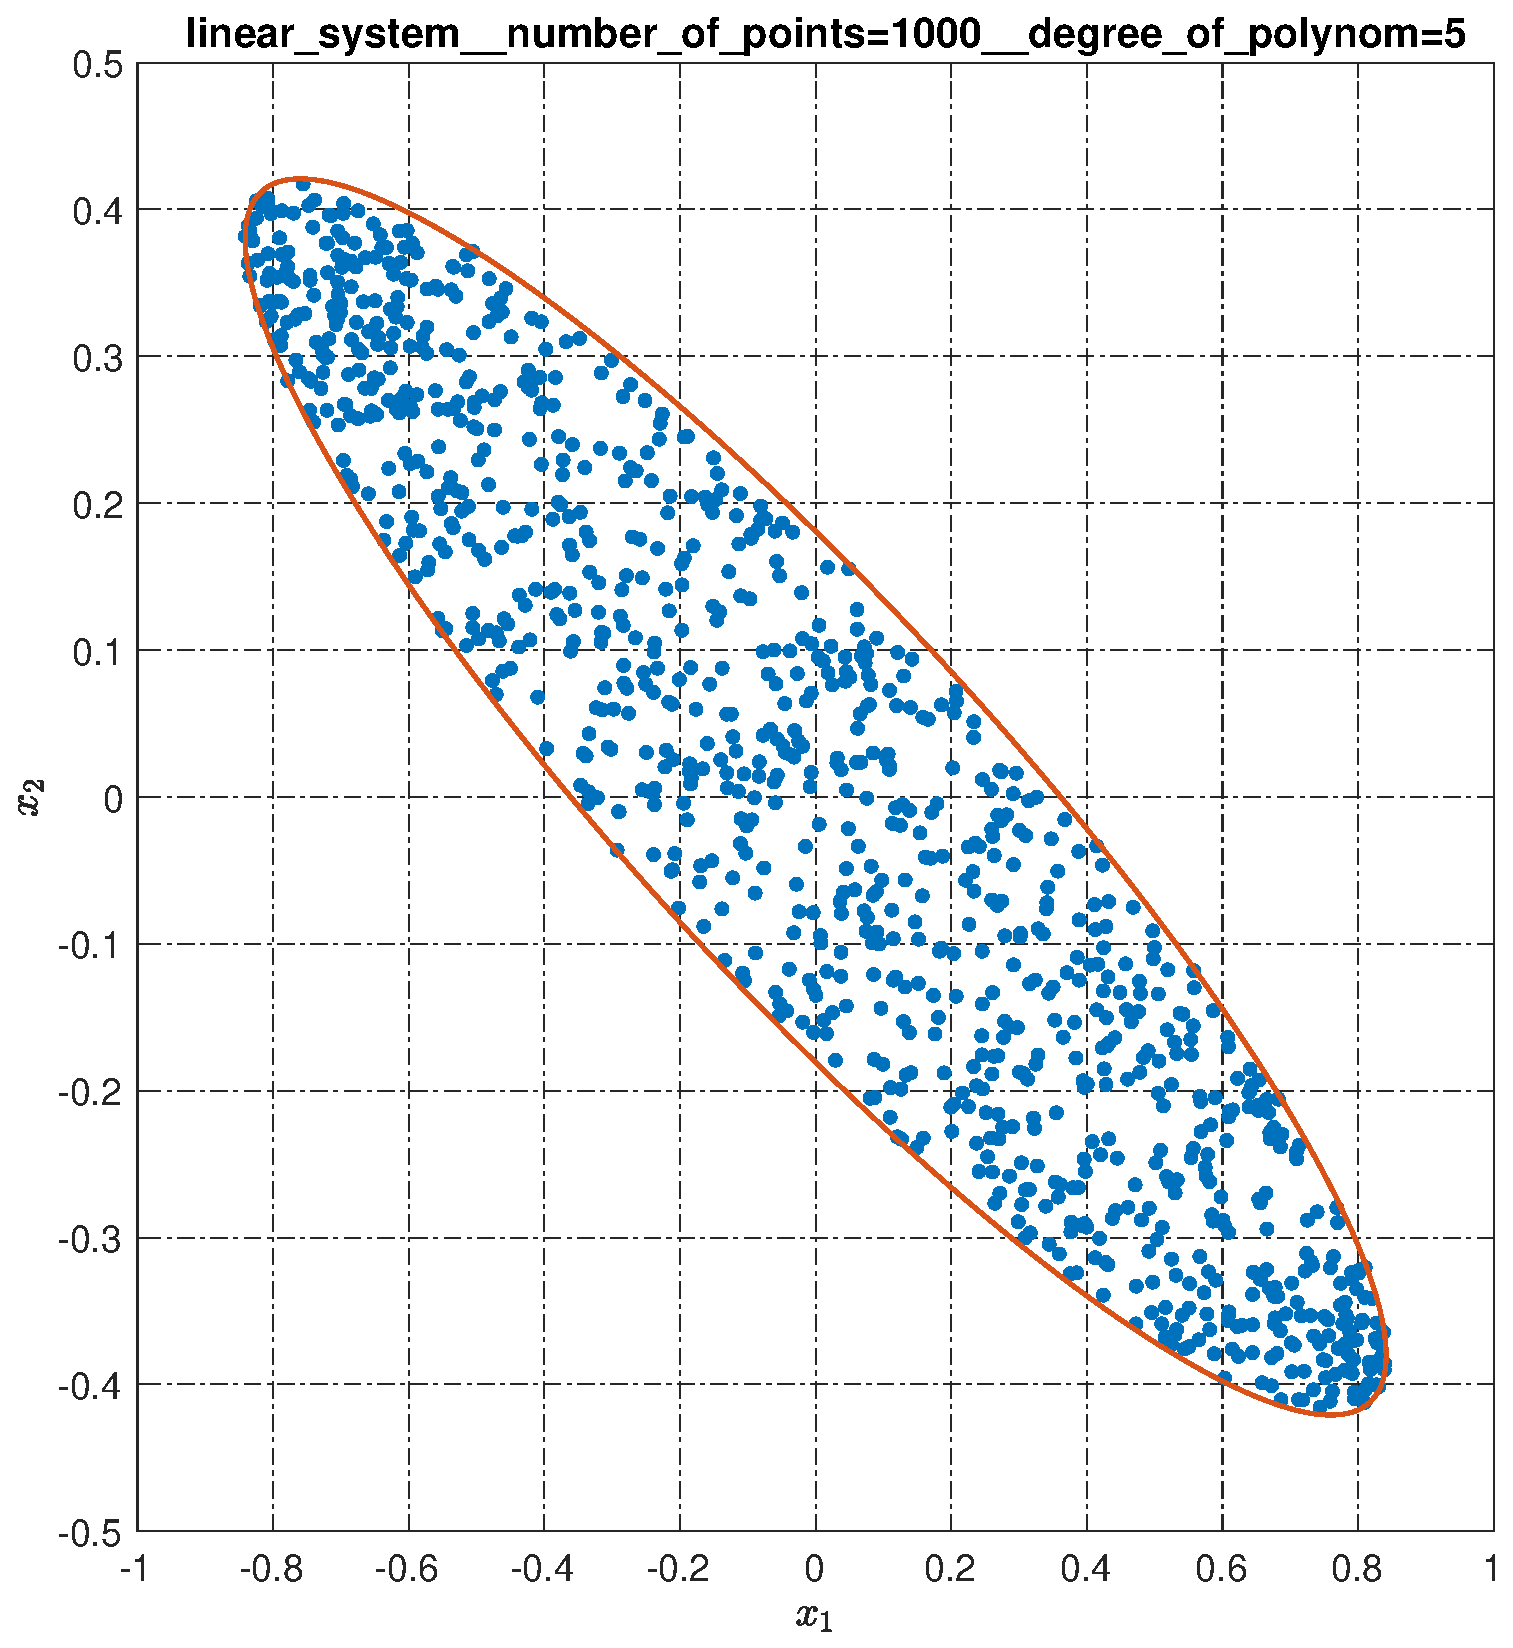
\includegraphics[width=\linewidth]{images/linear_system__number_of_points=1000__degree_of_polynom=5.eps}
  		\subcaption{$ N = 10^3 $ }
  	\end{minipage}
  	\hfill
  	\begin{minipage}[b]{.4\linewidth} 
  		\small
  		\centering
  		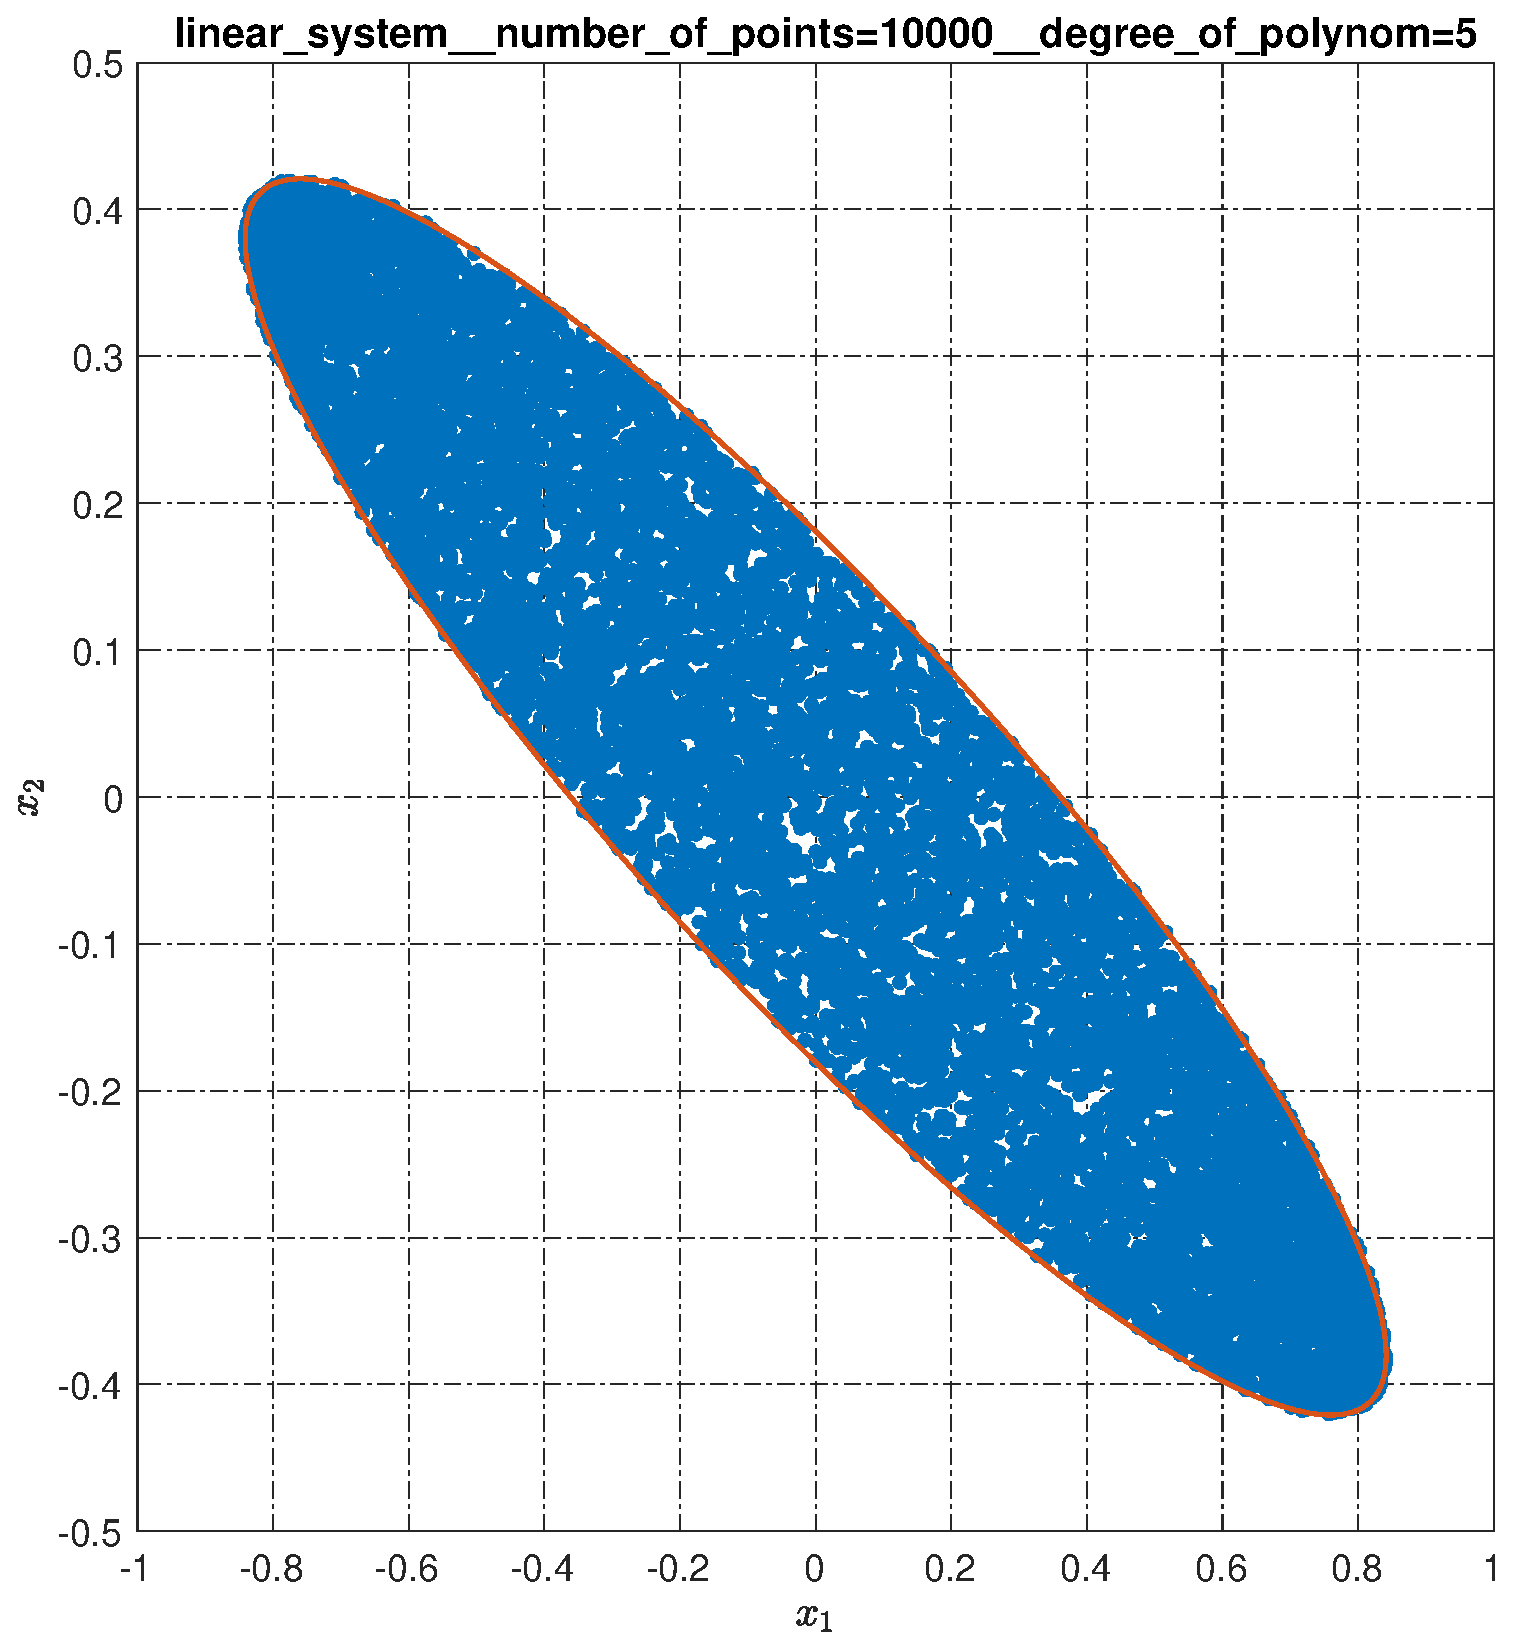
\includegraphics[width=\linewidth]{images/linear_system__number_of_points=10000__degree_of_polynom=5.eps}
  		\subcaption{$ N = 10^4  $ }
  	\end{minipage} 
  	\vfill
  	\hspace{-2.5ex}
  	\begin{minipage}[b]{.4\linewidth} 
  		\small
  		\centering 
  		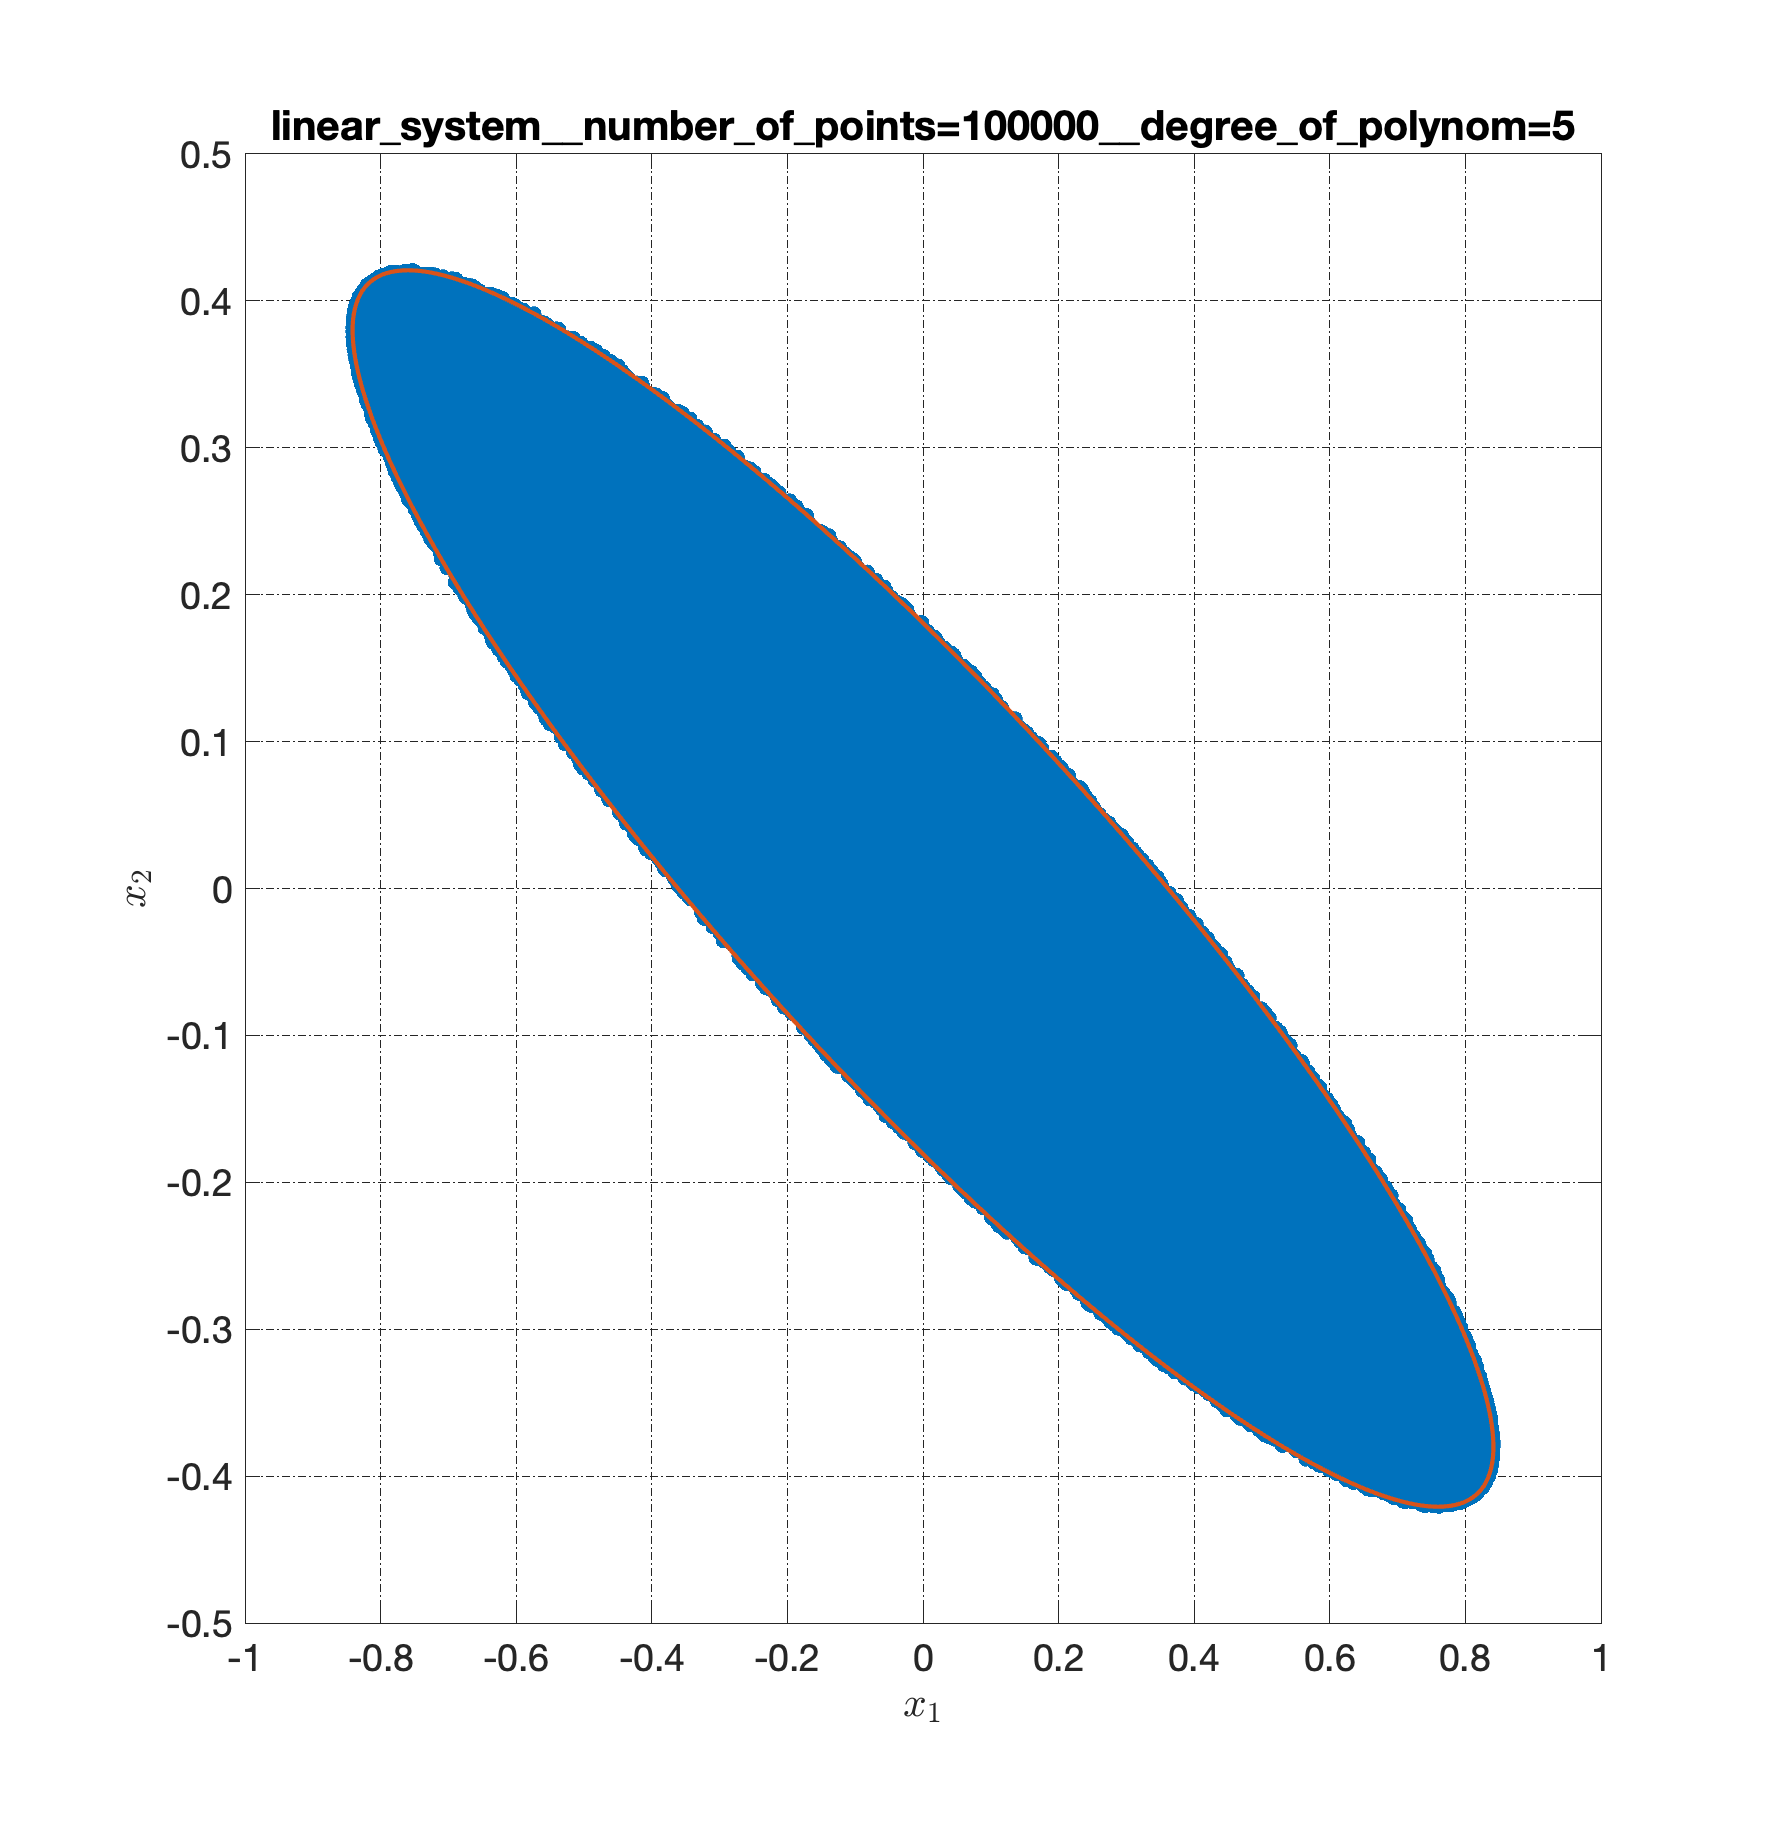
\includegraphics[width=\linewidth]{images/linear_system__number_of_points=100000__degree_of_polynom=5.eps}
  		\subcaption{$ N = 10^5  $ }
  	\end{minipage}
  	\hfill
  	\begin{minipage}[b]{.4\linewidth} 
  		\small
  		\centering
  		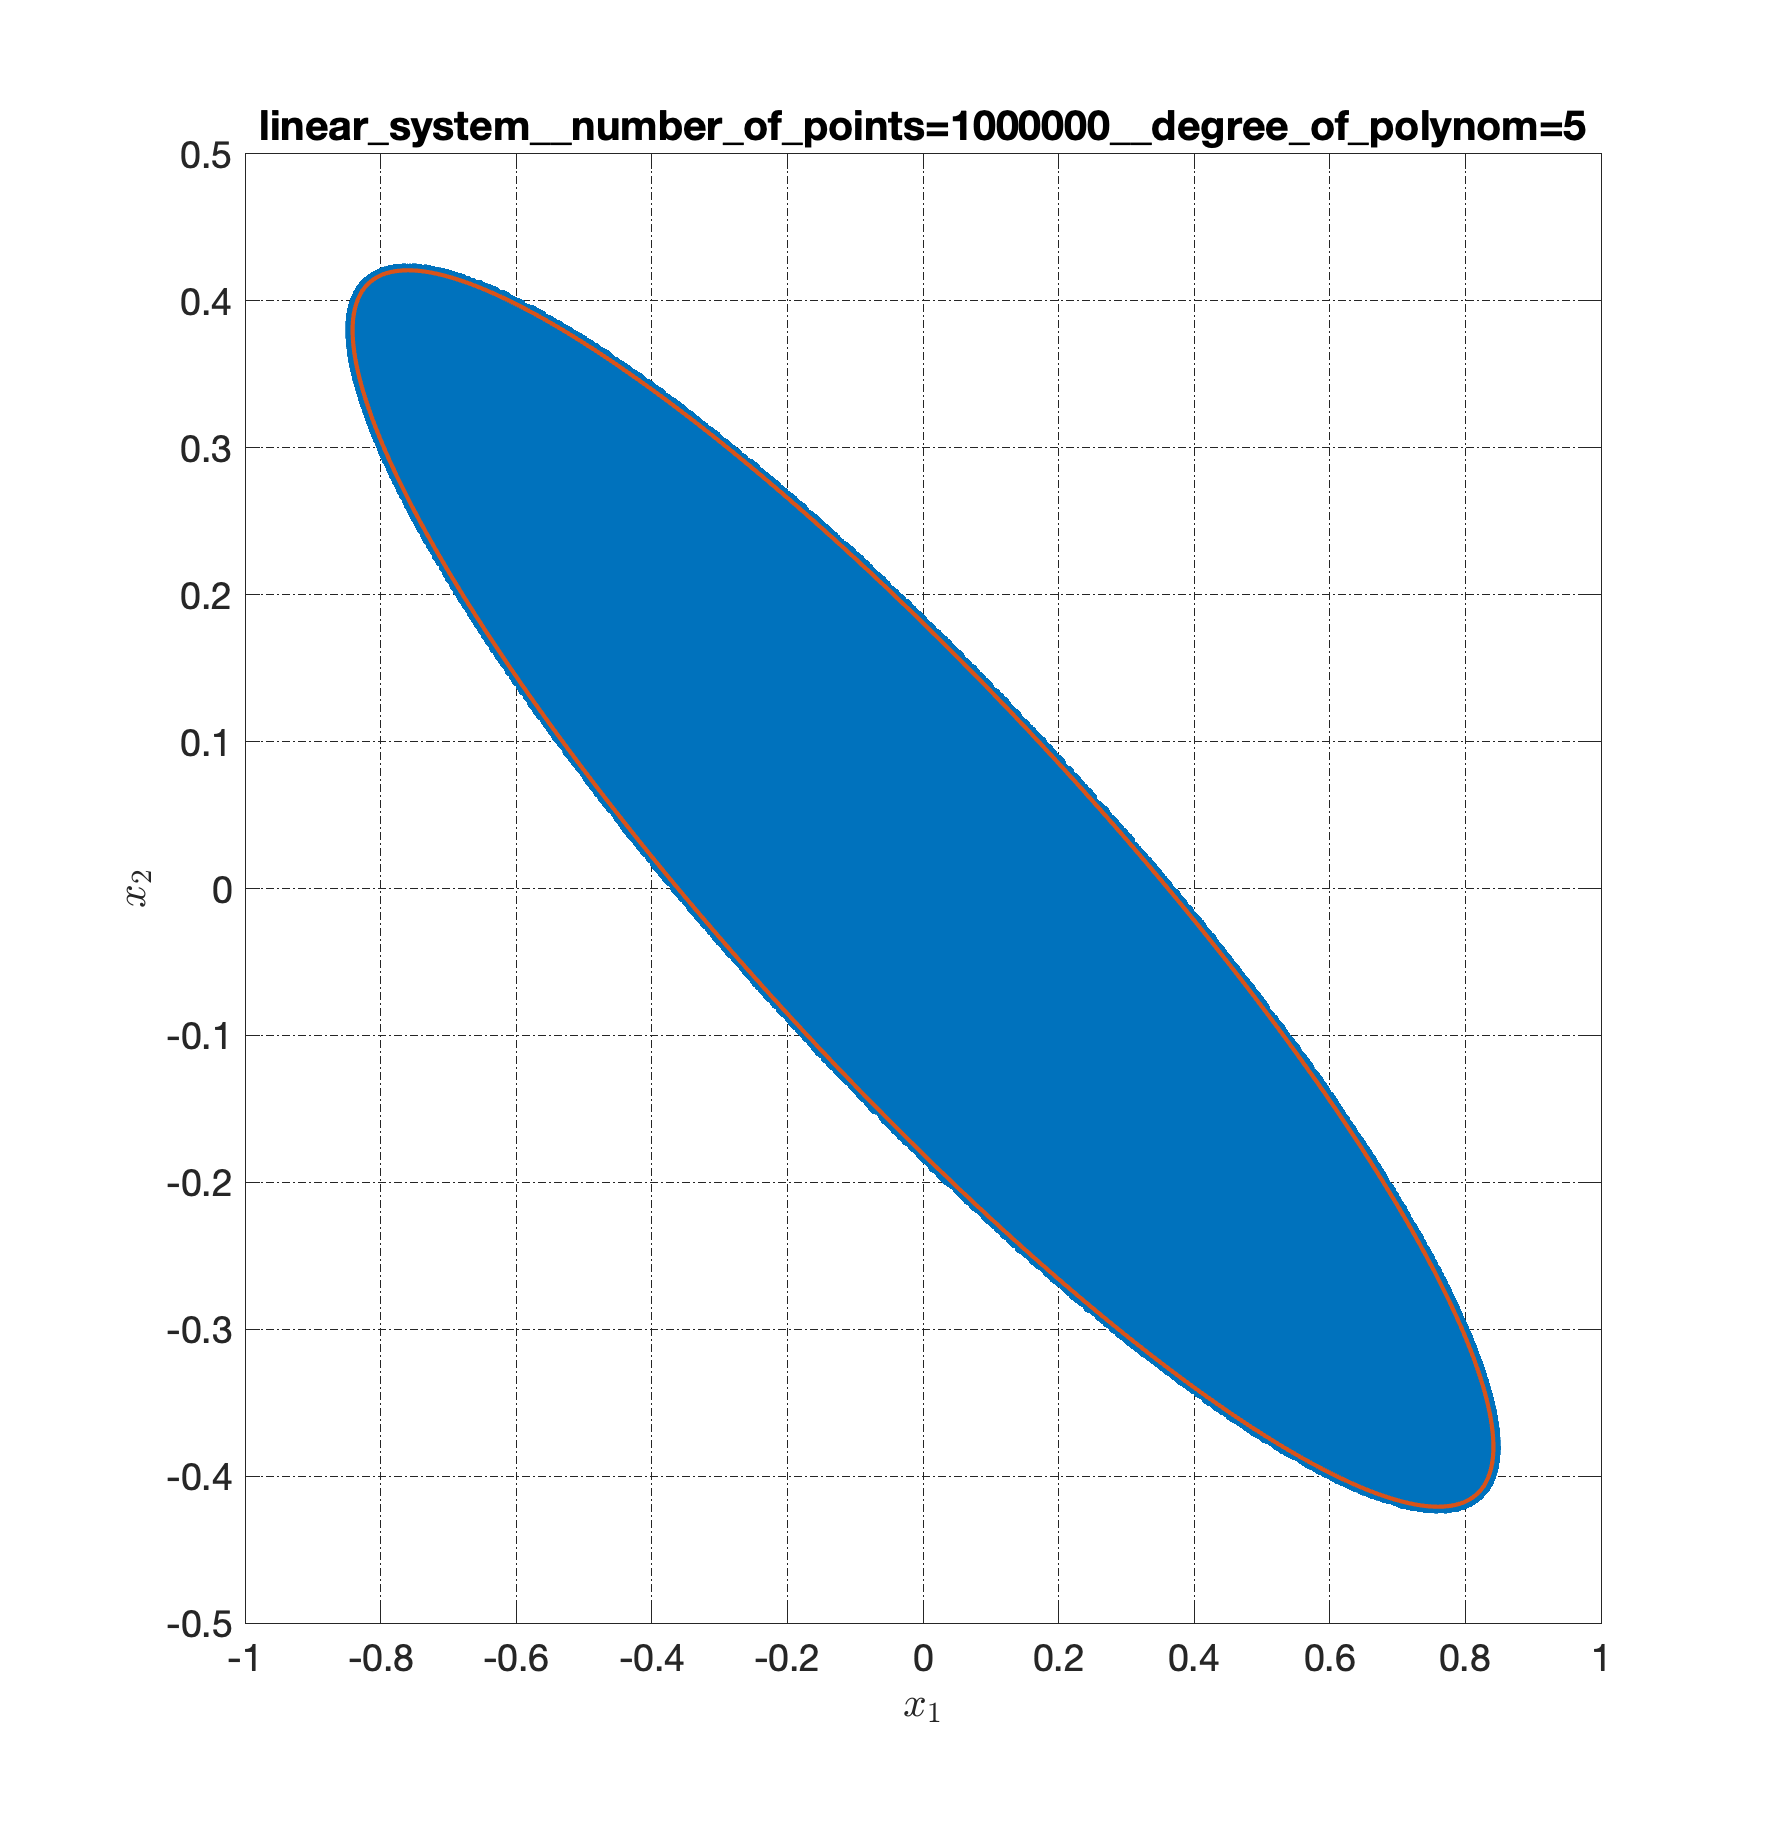
\includegraphics[width=\linewidth]{images/linear_system__number_of_points=1000000__degree_of_polynom=5.eps}
  		\subcaption{$ N = 10^6  $ } 
  	\end{minipage} 
  	\caption{Результаты численного эксперимента для системы \eqref{ap:linear_system1}.}\label{fig:ap:rs_linear1}
  \end{figure}
  \textbf{Линейная система.} На интервале времени $ 0 \leqslant t \leqslant 1$ рассмотрим линейную систему 
  \begin{gather}\label{ap:linear_system1}
  	\begin{pmatrix} 
  		\dot{x}_1 \\
  		\dot{x}_2  
  	\end{pmatrix} = 
  	\begin{pmatrix}
  		0 & 1 \\
  		-2 & -3
  	\end{pmatrix}
  	\begin{pmatrix} 
  		x_1 \\
  		x_2  
  	\end{pmatrix} +
  	\begin{pmatrix} 1 \\ 0
  	\end{pmatrix} u
  \end{gather}
  при нулевых начальных условиях $x_1(0) = x_2(0) = 0 $ и ограничениях на управление 
  \begin{gather*}
  	\int\limits_0^1 u^2dt \leqslant 1.
  \end{gather*}
  
  На рисунке \ref{fig:ap:rs_linear1} показаны множества достижимости системы \eqref{ap:linear_system1} при различных $N$.
  Красная линия --- граница множества достижимости, вычисленного аналитически.
  Видно, что при увеличении количестве точек, они заполняют множество достижимости.
  
   \begin{figure}[ht!] 
  	\hspace{-2.5ex}
  	\begin{minipage}[b]{.4\linewidth} 
  		\small
  		\centering 
  		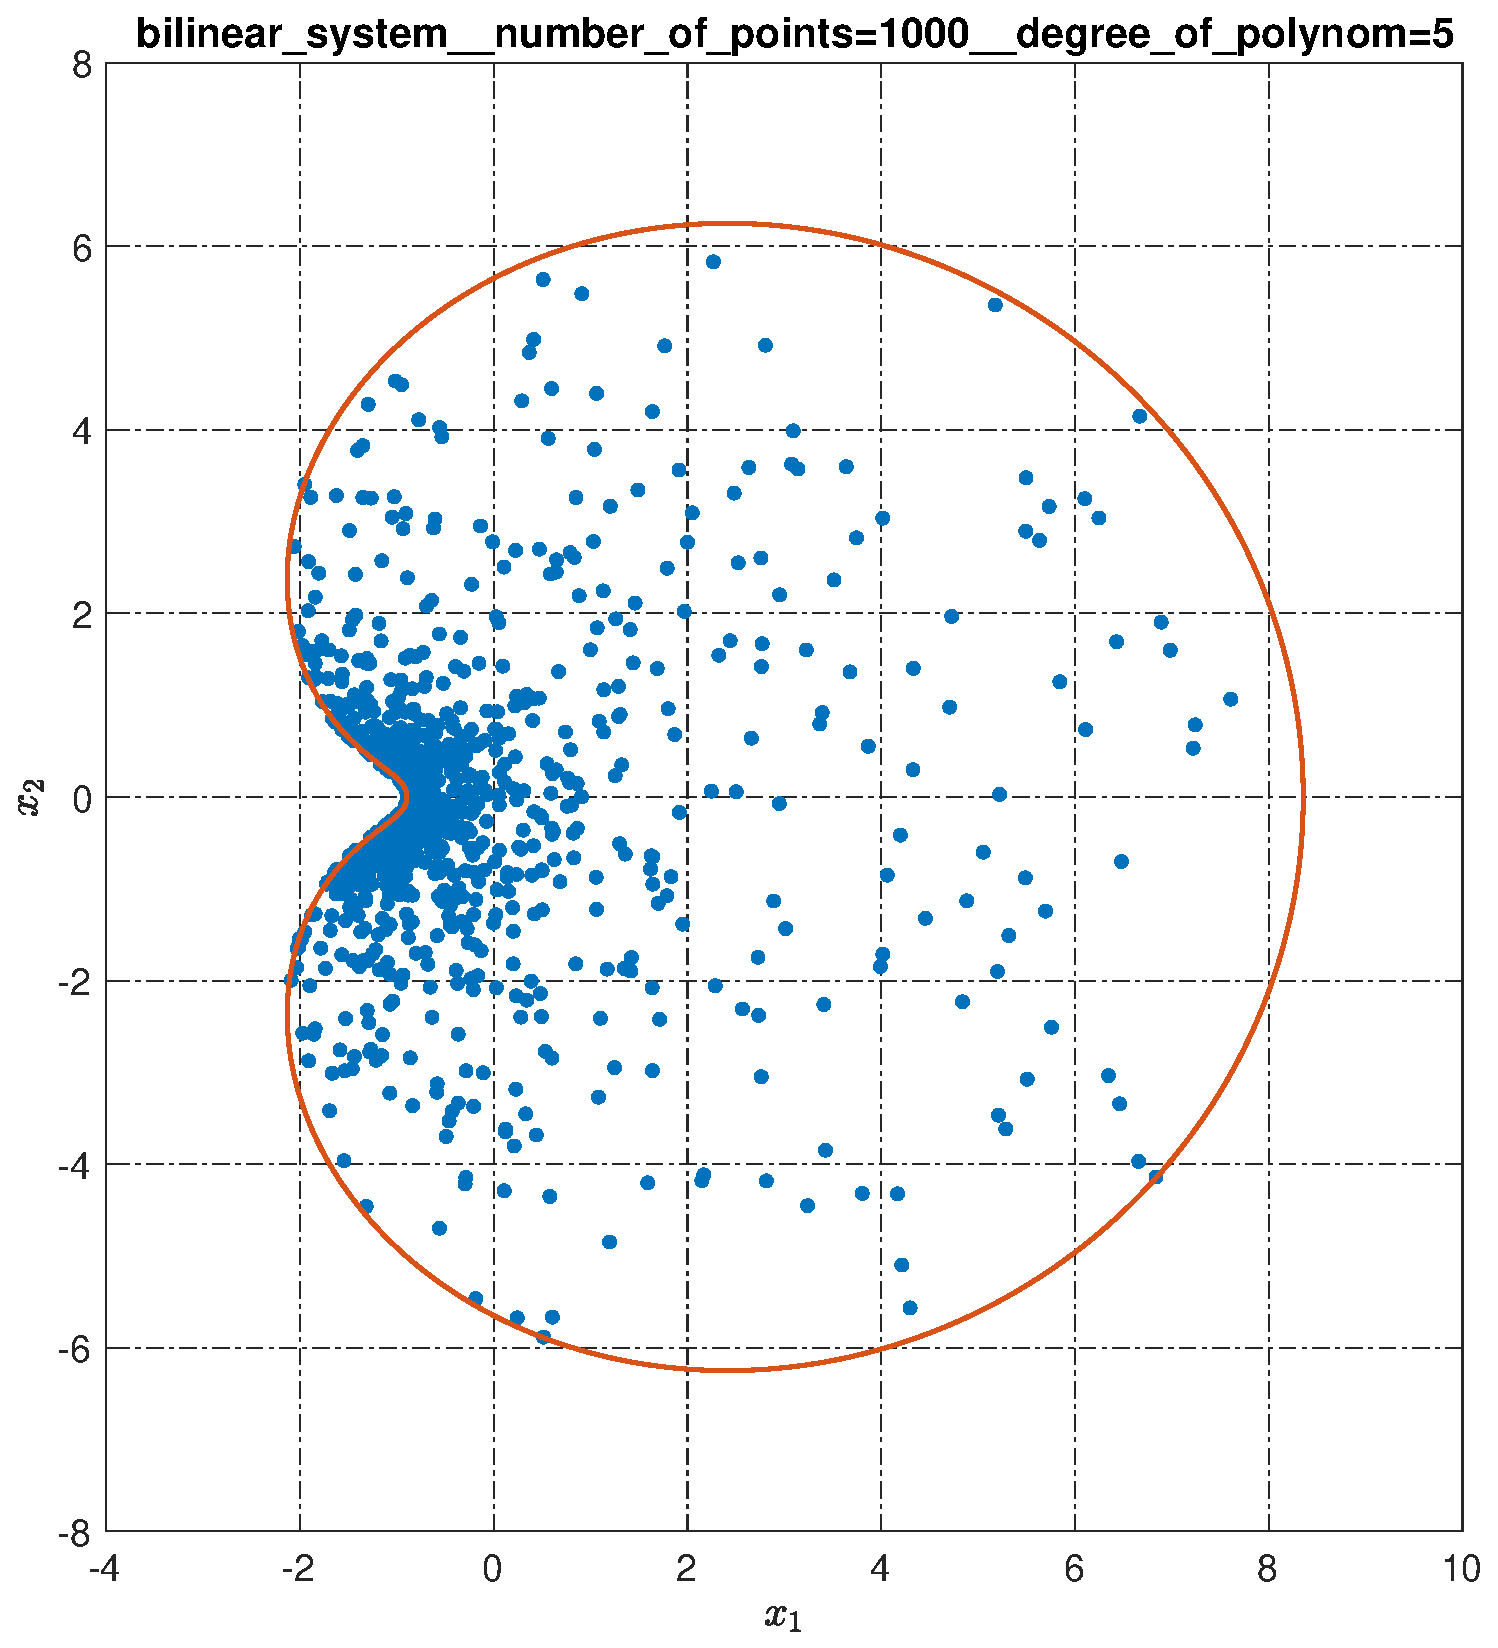
\includegraphics[width=\linewidth]{images/bilinear_system__number_of_points=1000__degree_of_polynom=5.eps}
  		\subcaption{$ N = 10^3  $ } 
  	\end{minipage}
  	\hfill
  	\begin{minipage}[b]{.4\linewidth} 
  		\small
  		\centering
  		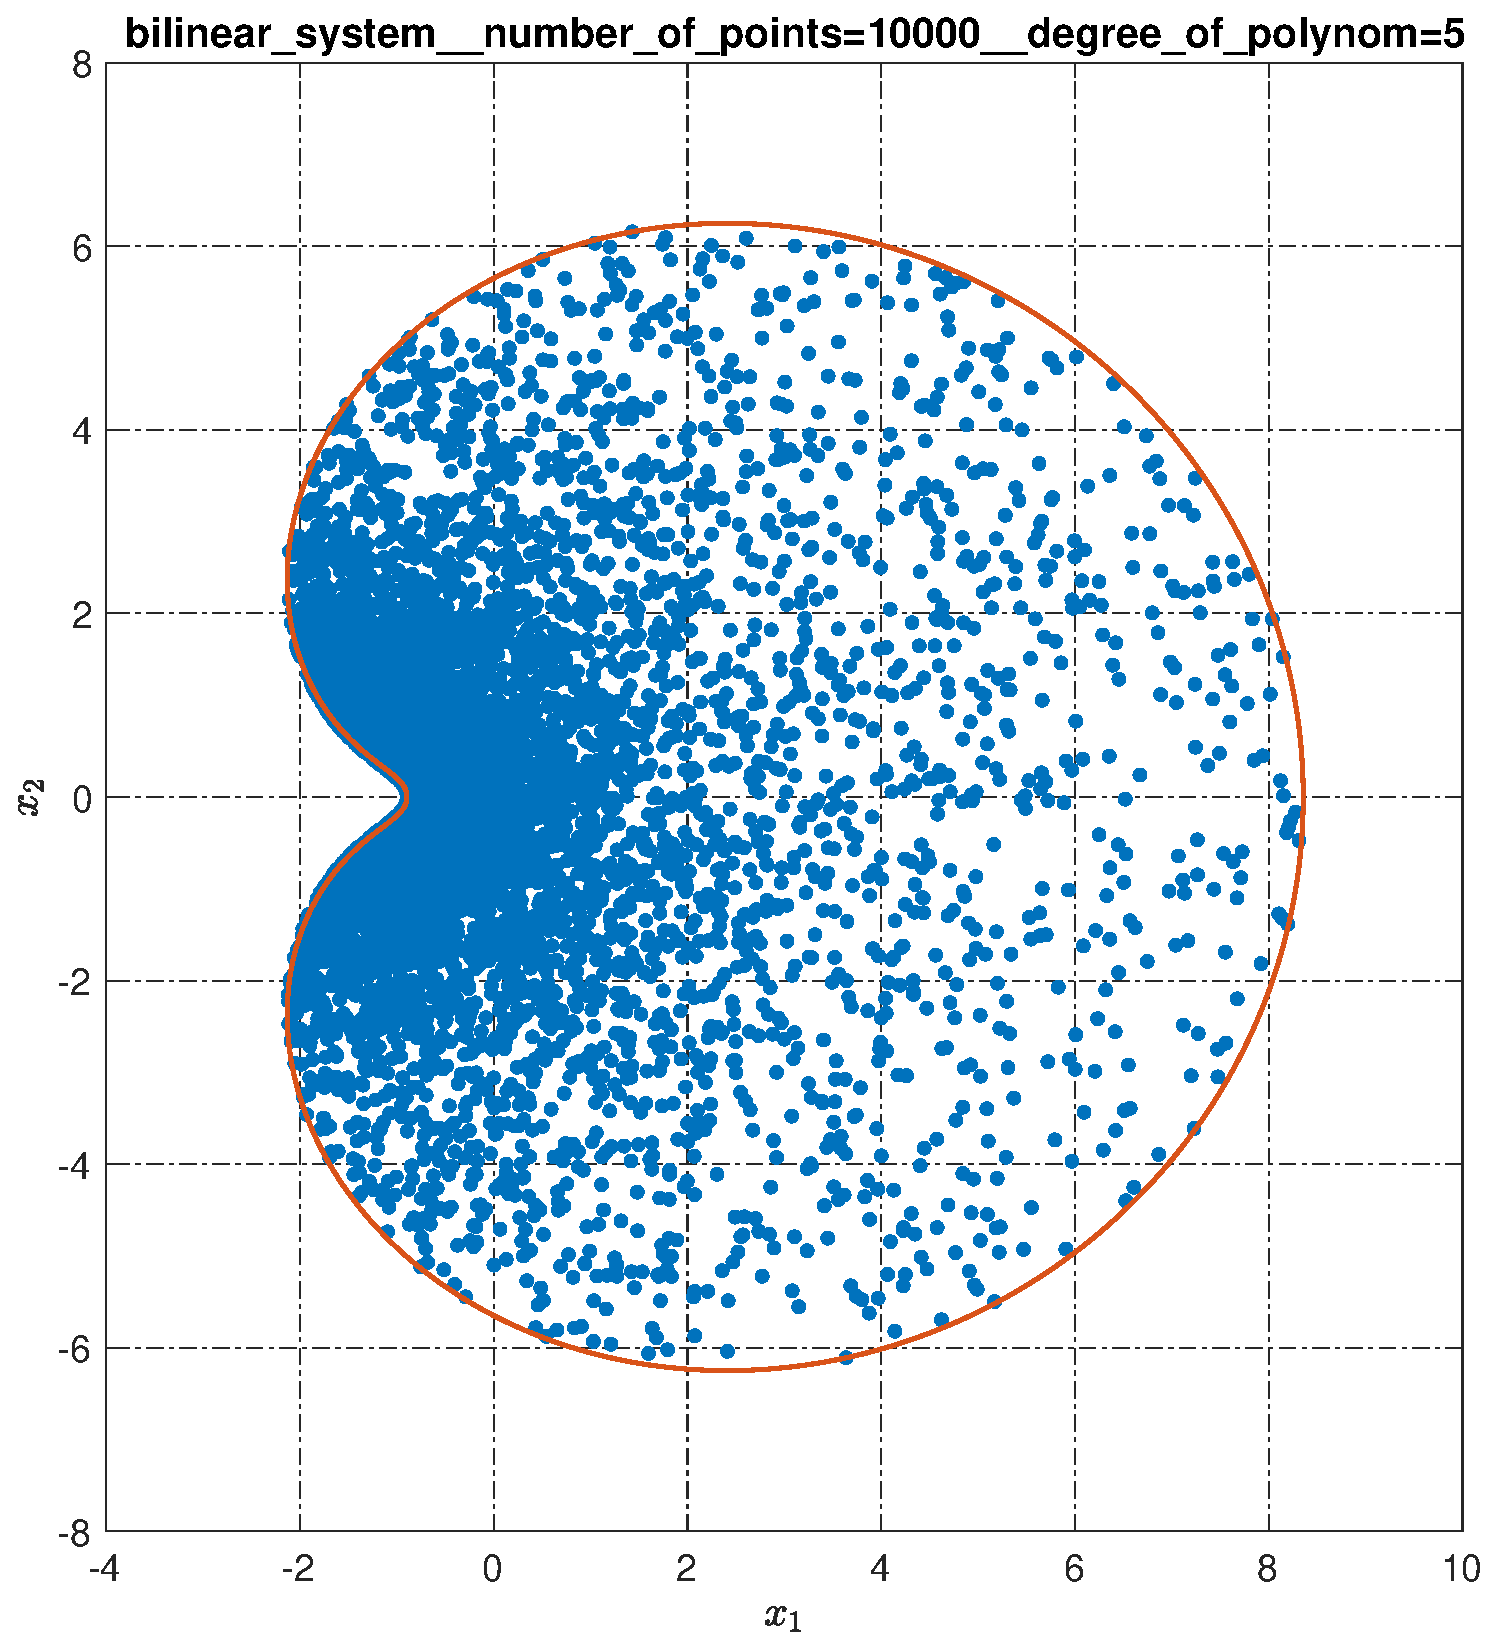
\includegraphics[width=\linewidth]{images/bilinear_system__number_of_points=10000__degree_of_polynom=5.eps}
  		\subcaption{$ N = 10^4  $ } 
  	\end{minipage} 
  	\vfill
  	\hspace{-2.5ex}
  	\begin{minipage}[b]{.4\linewidth} 
  		\small
  		\centering 
  		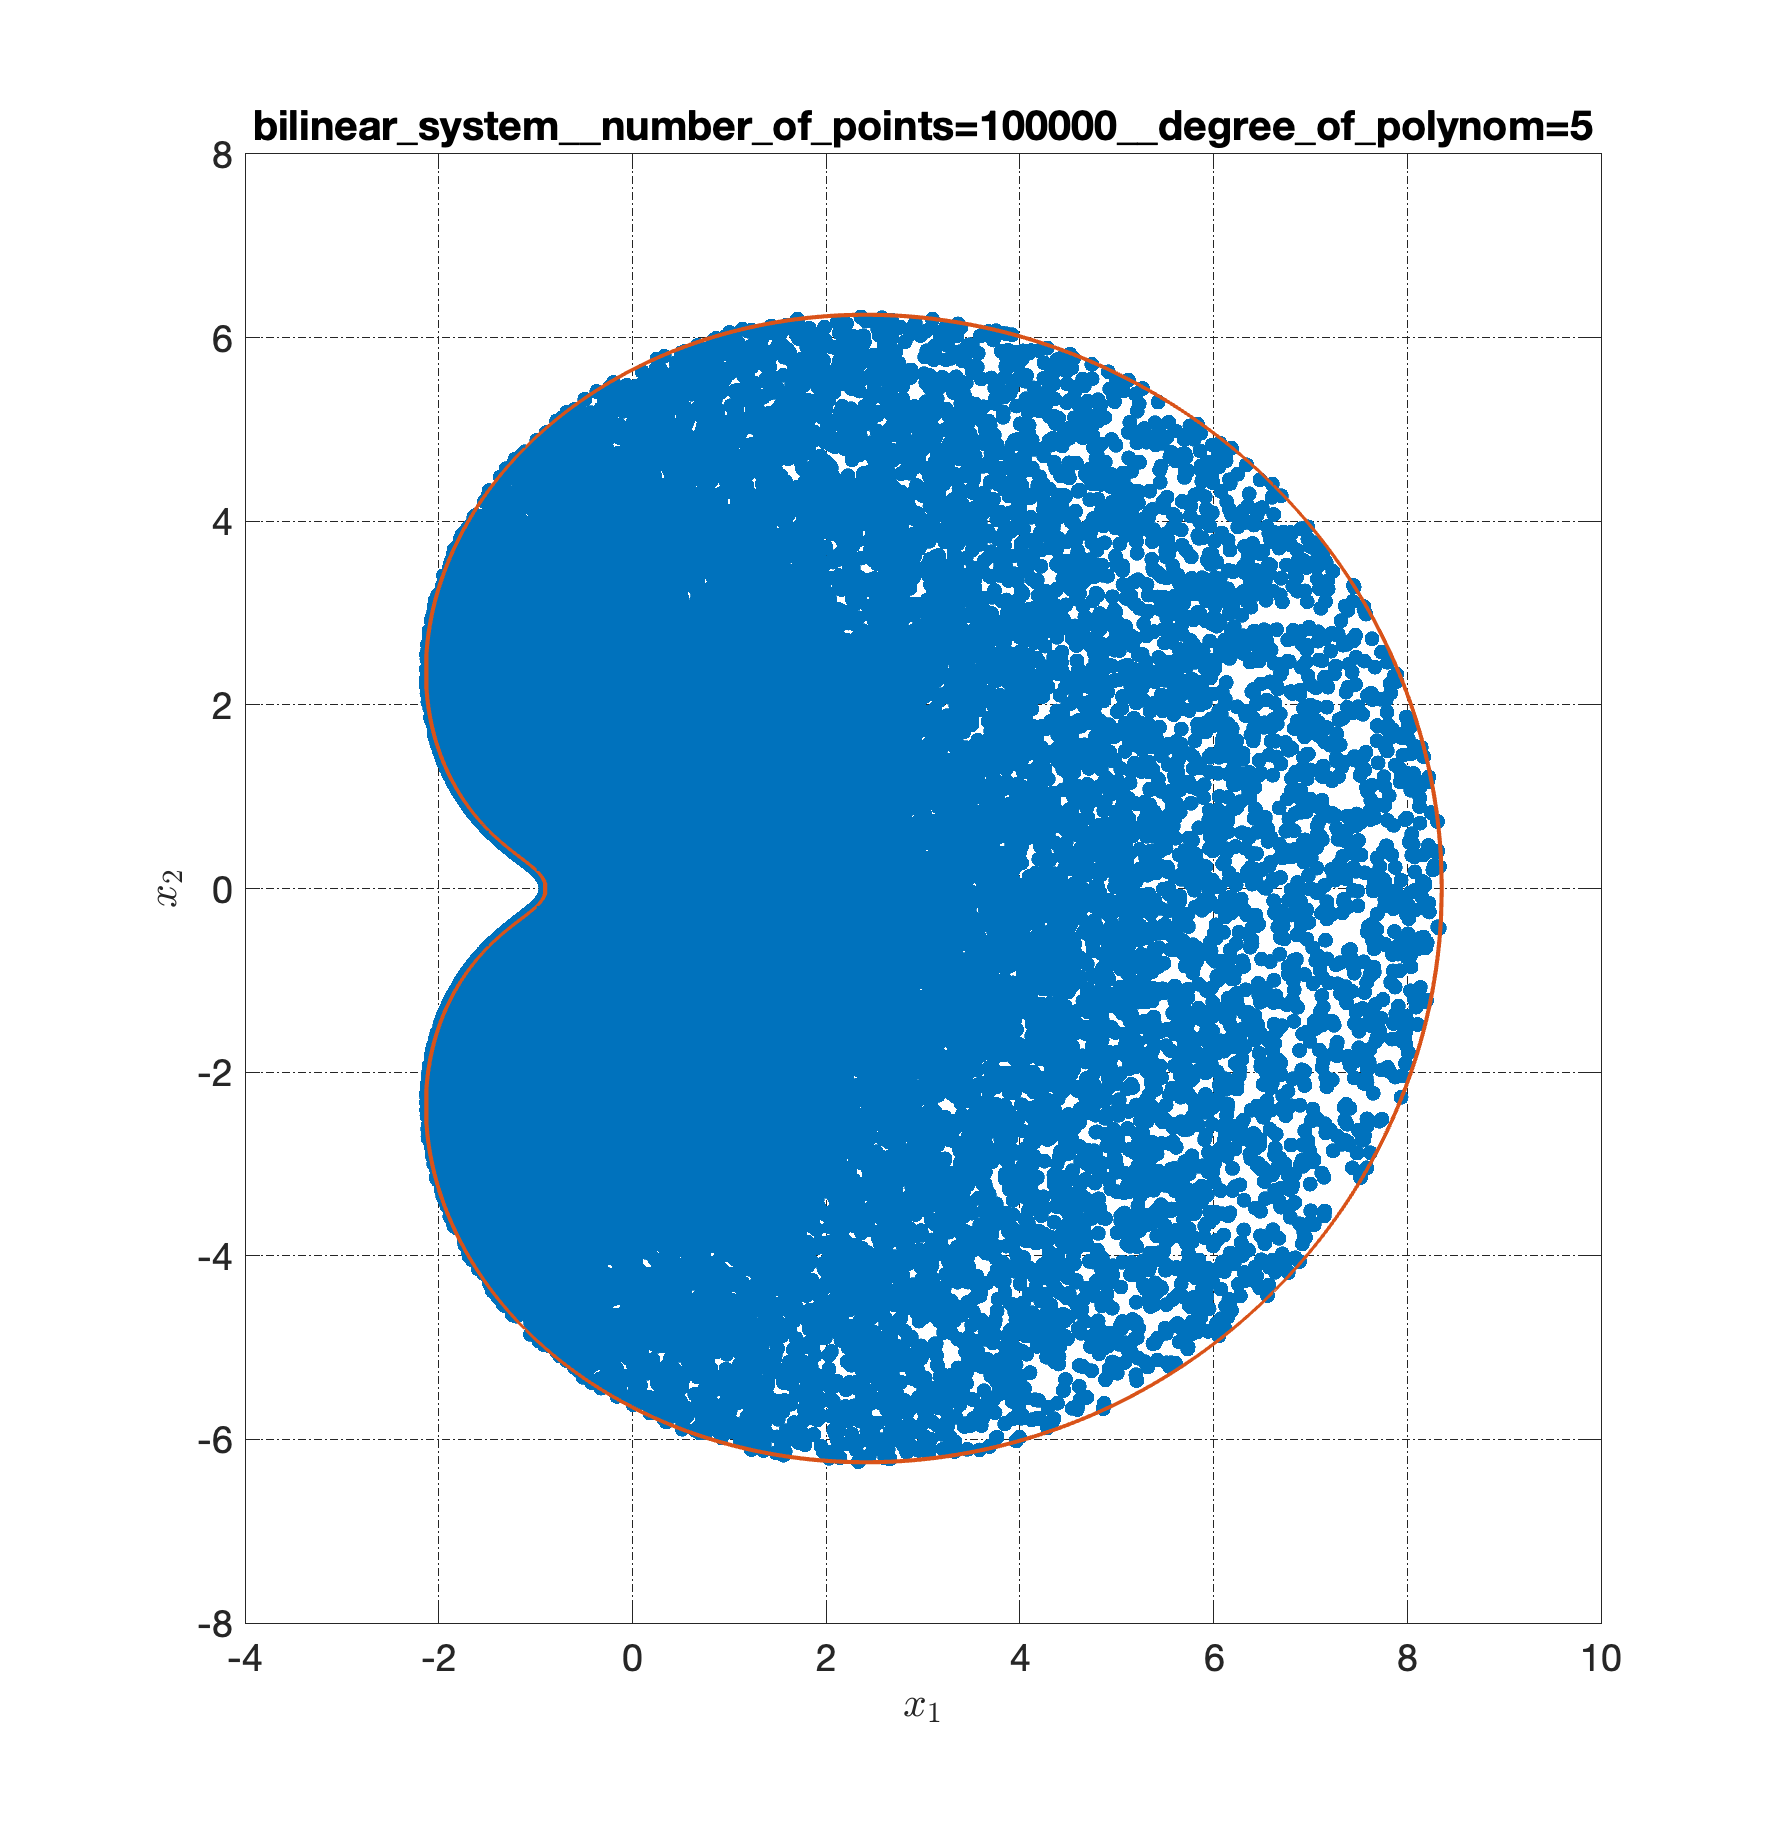
\includegraphics[width=\linewidth]{images/bilinear_system__number_of_points=100000__degree_of_polynom=5.eps}
  		\subcaption{$ N = 10^5  $ } 
  	\end{minipage}
  	\hfill
  	\begin{minipage}[b]{.4\linewidth} 
  		\small
  		\centering
  		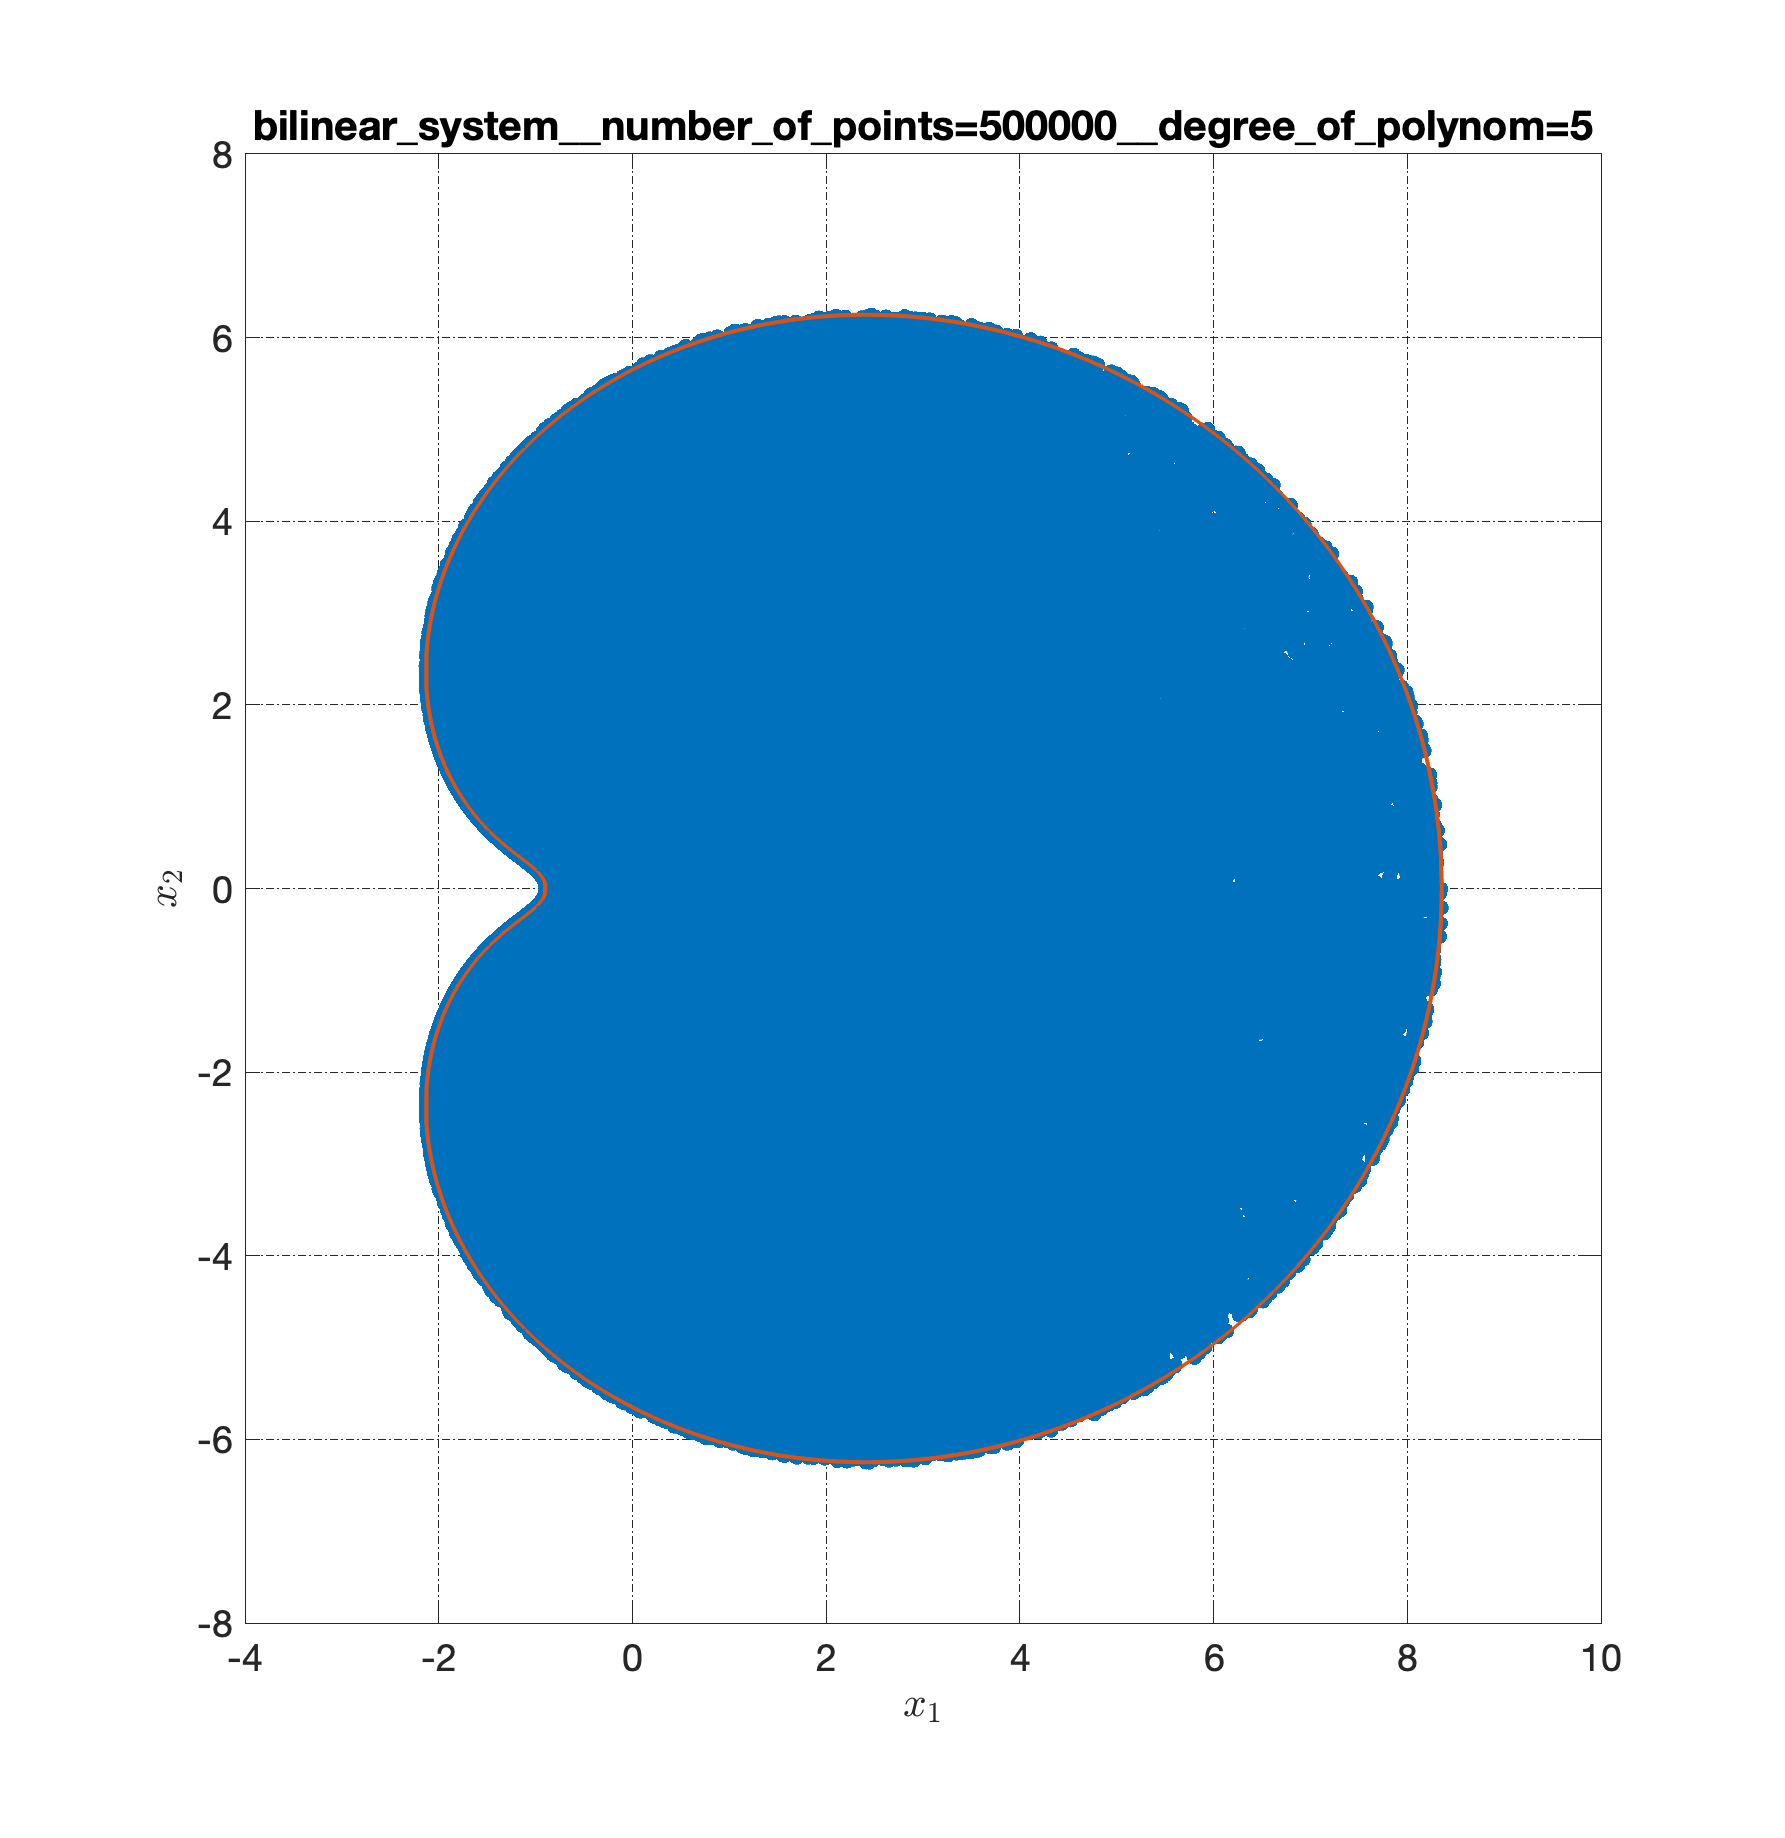
\includegraphics[width=\linewidth]{images/bilinear_system__number_of_points=500000__degree_of_polynom=5.eps}
  		\subcaption{$ N = 5\cdot10^5  $ } 
  	\end{minipage} 
  	\caption{Результаты численного эксперимента для системы \eqref{ap:nonlinear_system1}.}\label{fig:ap:rs_nonlinear1}
  \end{figure}
  
   \textbf{Нелинейная система.} В следующем примере рассмотрим нелинейную систему 
   \begin{gather}\label{ap:nonlinear_system1}
   	\begin{gathered}
   	\dot{x}_1 = x_2 u_1 - (1 + x_1) u_2,\\
   	\dot{x}_2 = -(1 + x_1) u_1 - x_2 u_2
   	\end{gathered}
   \end{gather}
   на интервале  $ 0 \leqslant t \leqslant 5$.
    Начальное состояние $x_1(0) = x_2(0) = 0 $, а управление стеснено такими же ограничениями, что и в прошлом примере
   \begin{gather*}
   	\int\limits_0^1 u^2dt \leqslant 1.
   \end{gather*}
   
     На рисунке \ref{fig:ap:rs_nonlinear1} показаны множества достижимости системы \eqref{ap:nonlinear_system1} при различных $N$.
       Красная линия --- граница множества достижимости, вычисленного аналитически.
   Видно, что при увеличении количества точек, они заполняют множество достижимости, однако, в отличии от линейной системы в предыдущем примере, здесь точки заполняют множество достижимости неравномерно.
   
     \begin{figure}[ht]
   	\centering
   	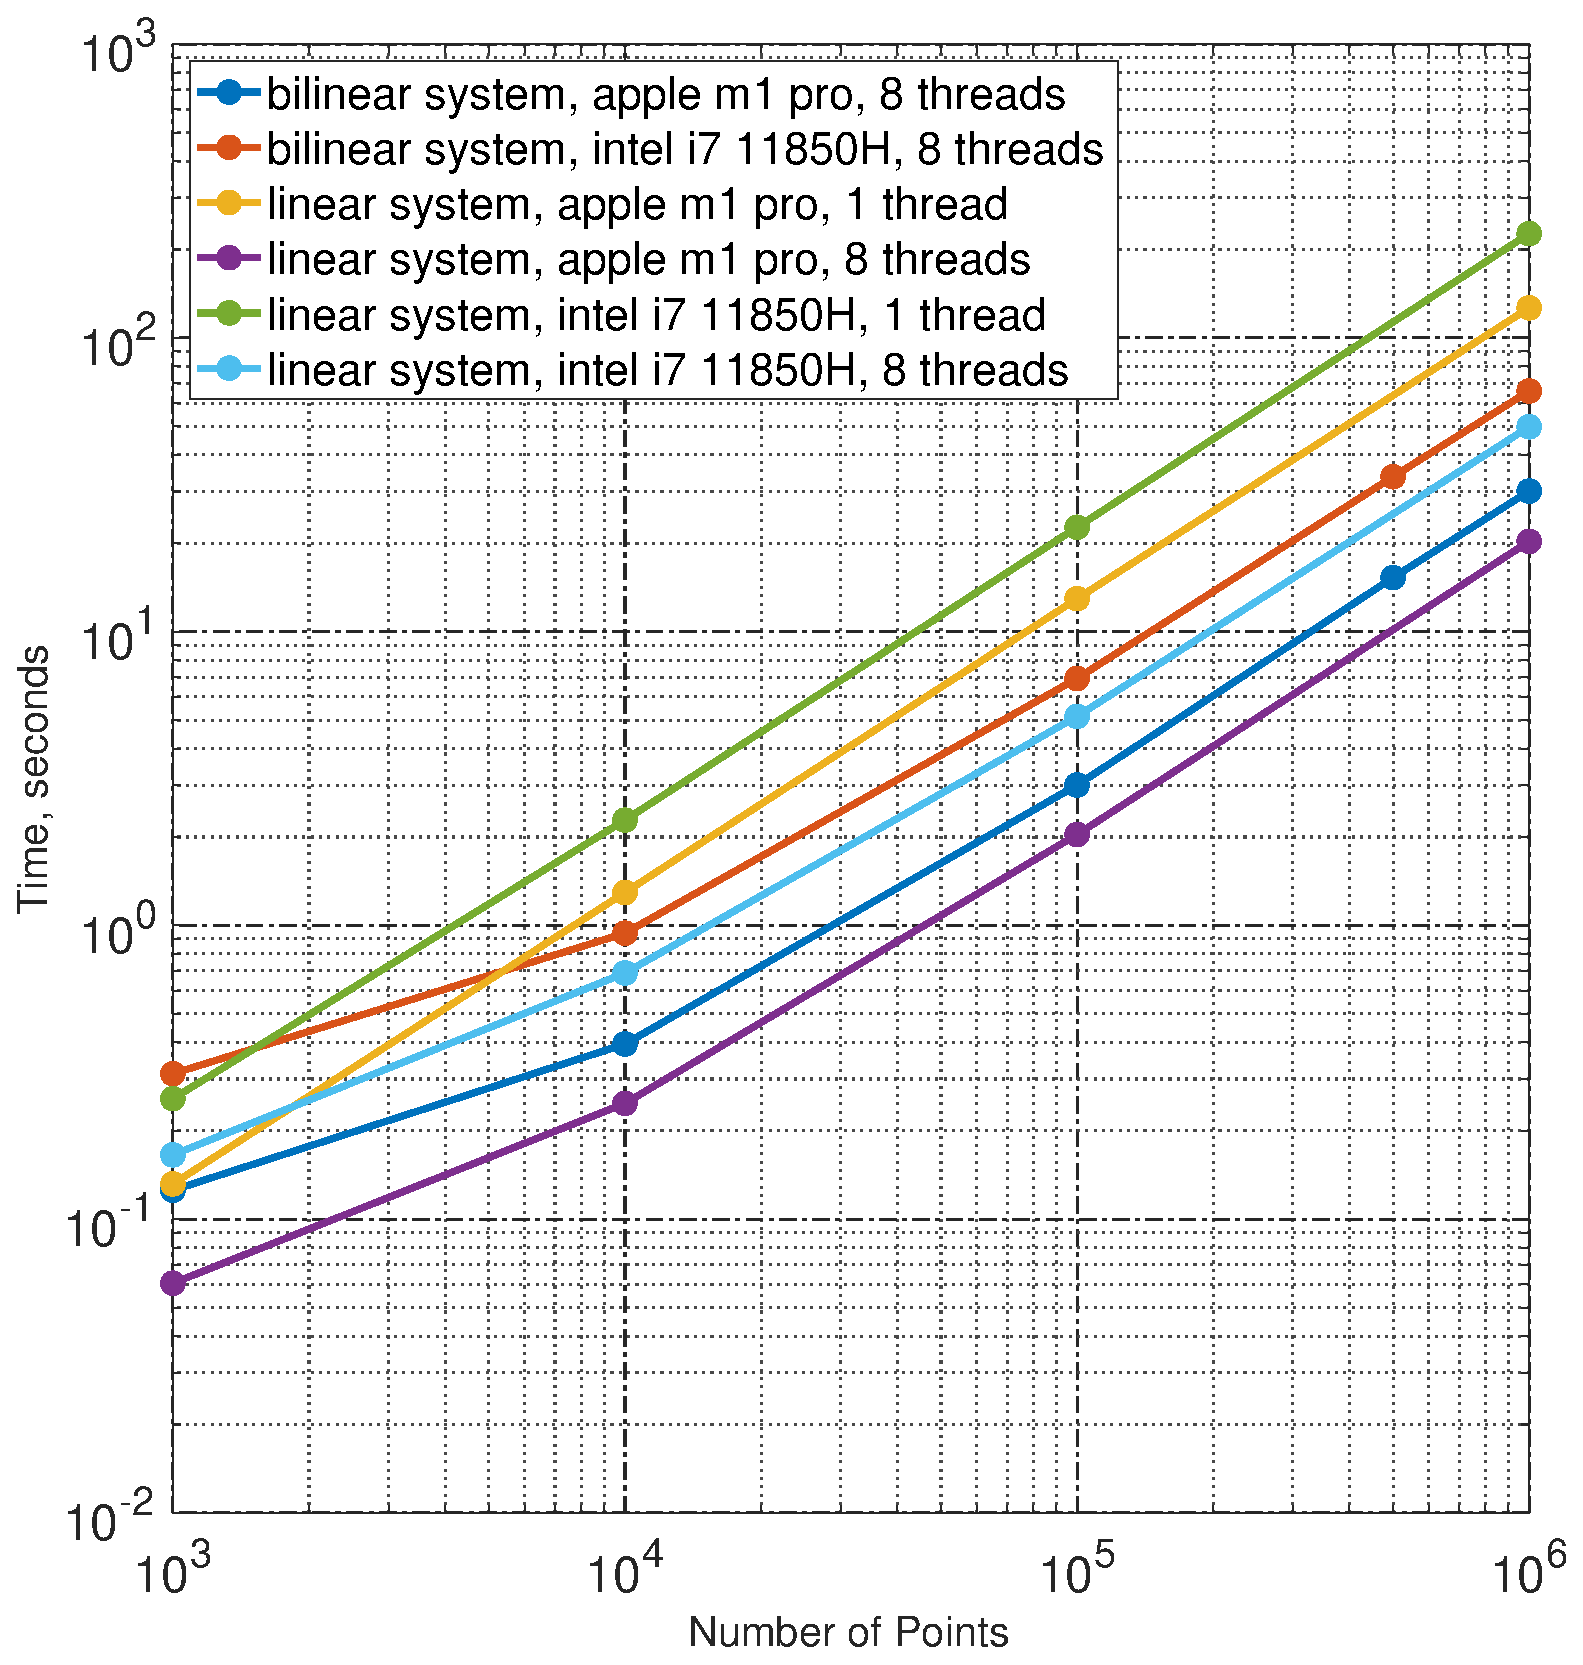
\includegraphics[width=0.5\textwidth]{images/time_complexity.eps}
   	\caption{Время работы алгоритма.}
   	\label{fig:ap:timings}
   \end{figure}
   
  Следующий рисунок, рисунок \ref{fig:ap:timings}, показывает зависимость времени работы алгоритм от количества точек. 
  Видно, что при параллельном вычисления точек множества достижимости время работы алгоритма существенно сокращается при постоянном количестве точек. 
  
  \subsection{Влияние выбора коэффициентов }
  
     \begin{figure}[ht]
  	\centering
  	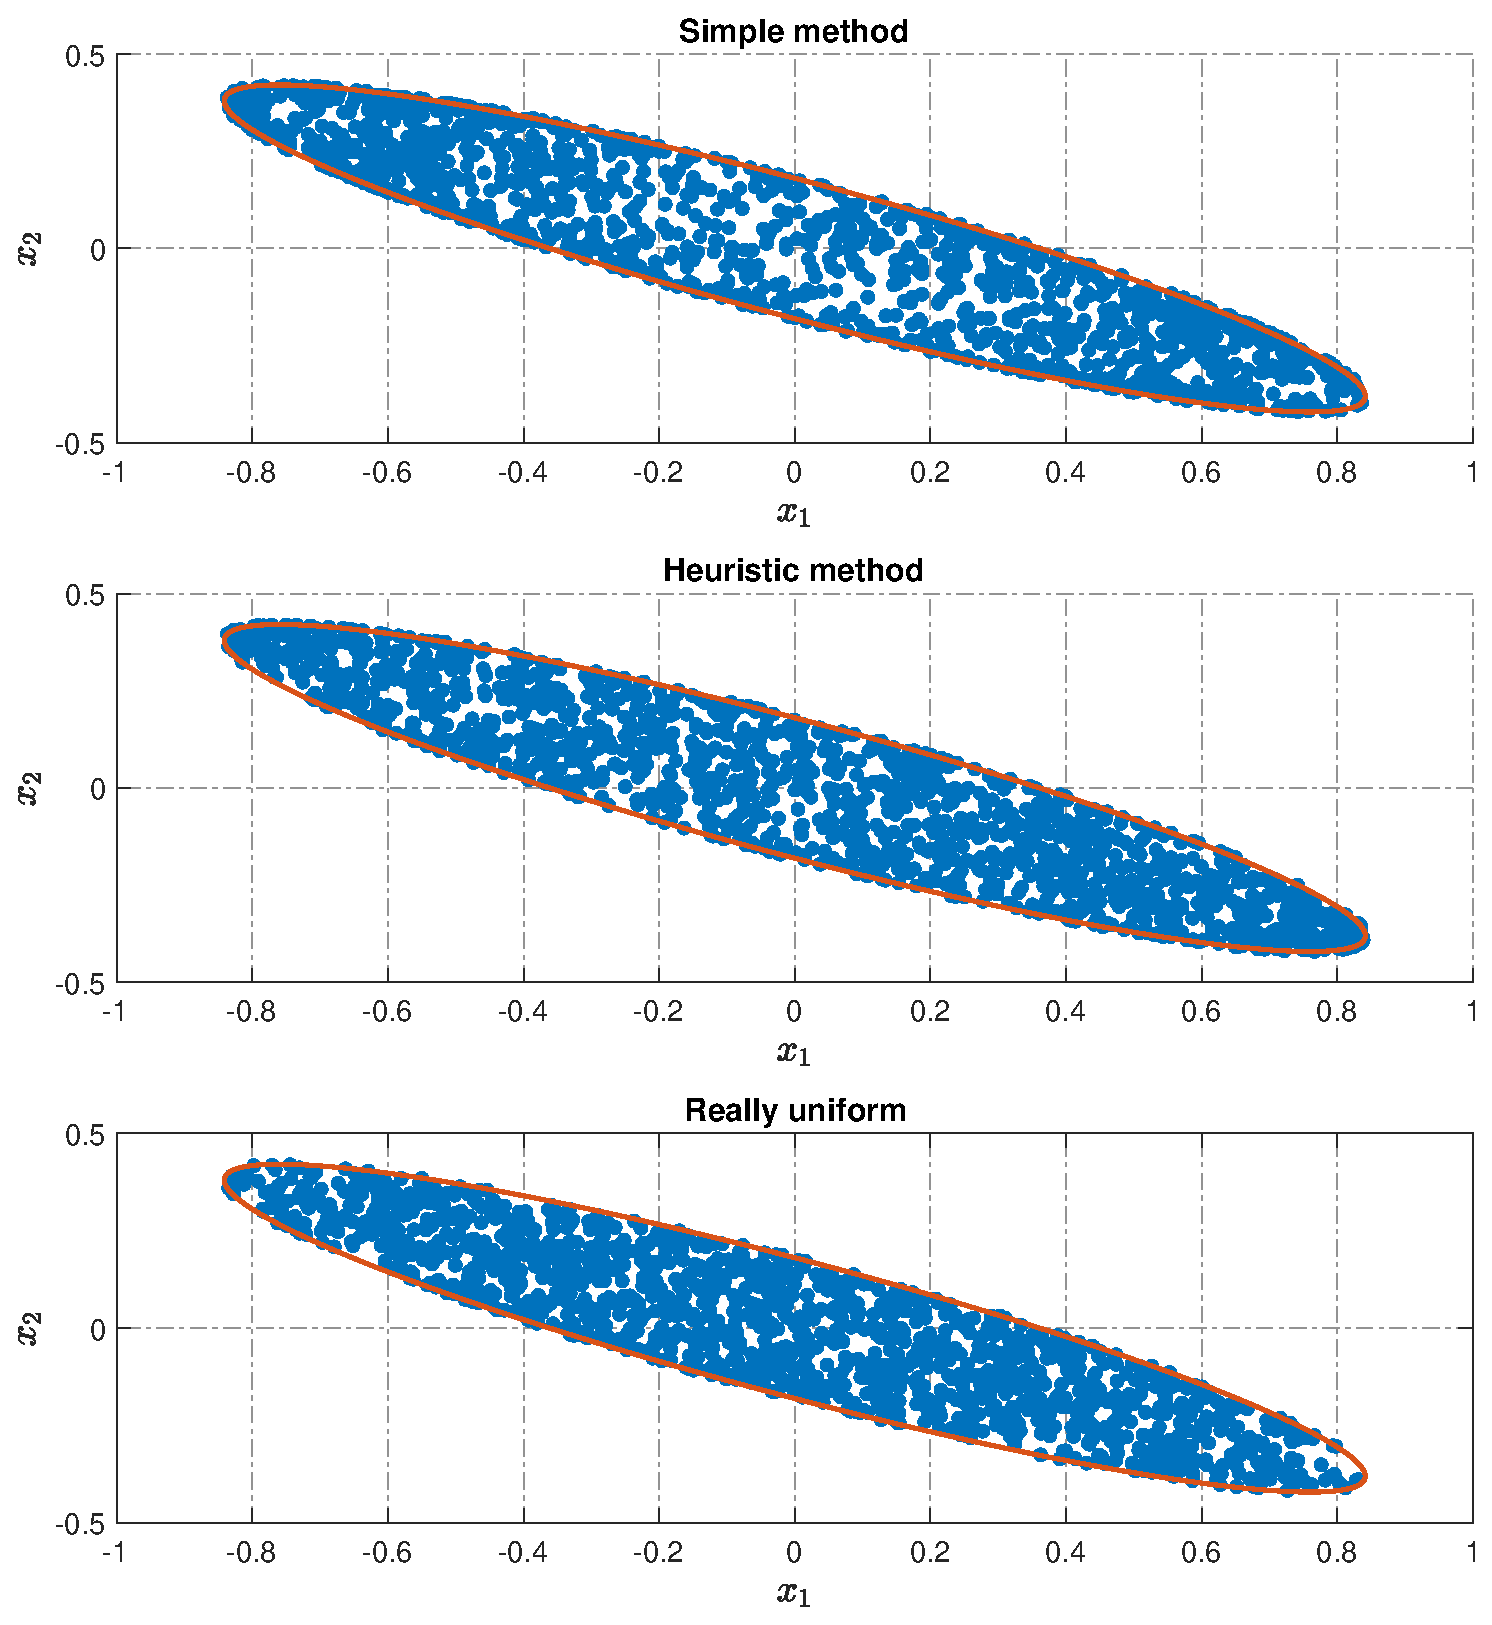
\includegraphics[width=0.5\textwidth]{images/three_linear_system_sets.eps}
  	\caption{Влияение выбора коэффициентов $C_i$.}
  	\label{fig:ap:coeffs_RS}
  \end{figure}
  
  Оказалось, что равномерность заполнения множеств достижимости точками сильно зависит от выбора коэффициентов $C_i$. 
  Автор использовал два метода получения случайной матрицы $C_i \in \mathbb{R}^{r \times k+1}$  с заданной фробениусовой нормой $ \|C_i\| = \mu$. 
  
  Первый метод состоит в генерации $r (k + 1)$ равномерно распределенных скаляров $\overline{c}_{i, j} \sim U[-1;1]$, $ j = 1\dots r (k + 1)$, составлении из них матрицы $\overline{C_i}  \in \mathbb{R}^{r \times k+1}$ и нормировании ее
  \begin{gather*}
  		C_i = \frac{\mu}{\|C_i\|}\overline{C_i}.
  \end{gather*}
  
  В верхней части рисунка \ref{fig:ap:coeffs_RS} представлено множество достижимости системы \eqref{ap:linear_system1} полученное с использованием этого метода генерации коэффициентов. 
 
  Второй метод также состоит из покомпонентной генерации равно распределенных скаляров, однако, диапазон в котором происходит генерация уменьшается на сумму квадратов уже сгенерированных компонентов.   
  Так, нулевой компонент $c_{i, 0}$ равномерно распределен в диапазоне $[-\mu; \mu]$, $c_{i, 0} \sim U[-\mu; \mu]$. 
  Первый компонент выбирается 
  \begin{gather*}
  	 c_{i, 1} \sim U\left[-\sqrt{\mu^2 - c_{i, 0}^2}; \sqrt{\mu^2 - c_{i, 0}^2}\right].
  \end{gather*} 
  Аналогично выбираются все остальные компоненты, кроме последнего
    \begin{gather*}
  	c_{i, j} \sim U\left[-\sqrt{\mu^2 - \sum\limits_{s = 0}^j c_{i, s}^2}; \sqrt{\mu^2 - \sum\limits_{s = 0}^j c_{i, s}^2}\right], \qquad 1 \leqslant j \leqslant r(k+1) - 2.
  \end{gather*} 
  Величина последнего коэффициента выбирается равной $\sqrt{\mu^2 - \sum\limits_{s = 0}^{r(k+1) - 2} c_{i, s}^2} $, а случайно выбирается лишь его знак.
  На рисунке \ref{fig:ap:coeffs_RS} приведено три результата генерации одинакового количества точек множества достижимости системы \eqref{ap:linear_system1}.
  На верхнем рисунке показан результат использования первого метода генерации коэффициентов, в среднем рисунке использован второй метод, а в нижней части рисунка, аналитически рассчитанный эллипсоид множества достижимости равномерно заполнен таким же количеством точек, как и в первых двух частях рисунка. 
  Видно, что в верхней части рисунка эллипсоид заполнен менее равномерно, чем в средней и тем более, чем в нижней. 
  
  Для того, чтобы исследовать причины такого результата, решим обратную задачу, восстановив управления, ведущие в равномерно распределенные точки третьего рисунка и коэффициенты разложения этих управлений по той же системе полиномов третьего порядка, что и использовалась в первых двух рисунках.
  
  Точки множества достижимости, полученные в результате работы Алгоритма \ref{ap:method} можно представить в виде $x_i(T, u_i) = M C_i^{\top}$, где $M$ --- матрица, составленная из решений системы \eqref{ap:linear_system1}, порожденных управлениями в виде полиномов $p_k(t)$, 
  \begin{gather}
  	 M = \big(x(T, p_0), x(T, p_1), \dots, x(T, p_k)\big).
  \end{gather} 
  
    \begin{figure}[ht]
  	\centering
  	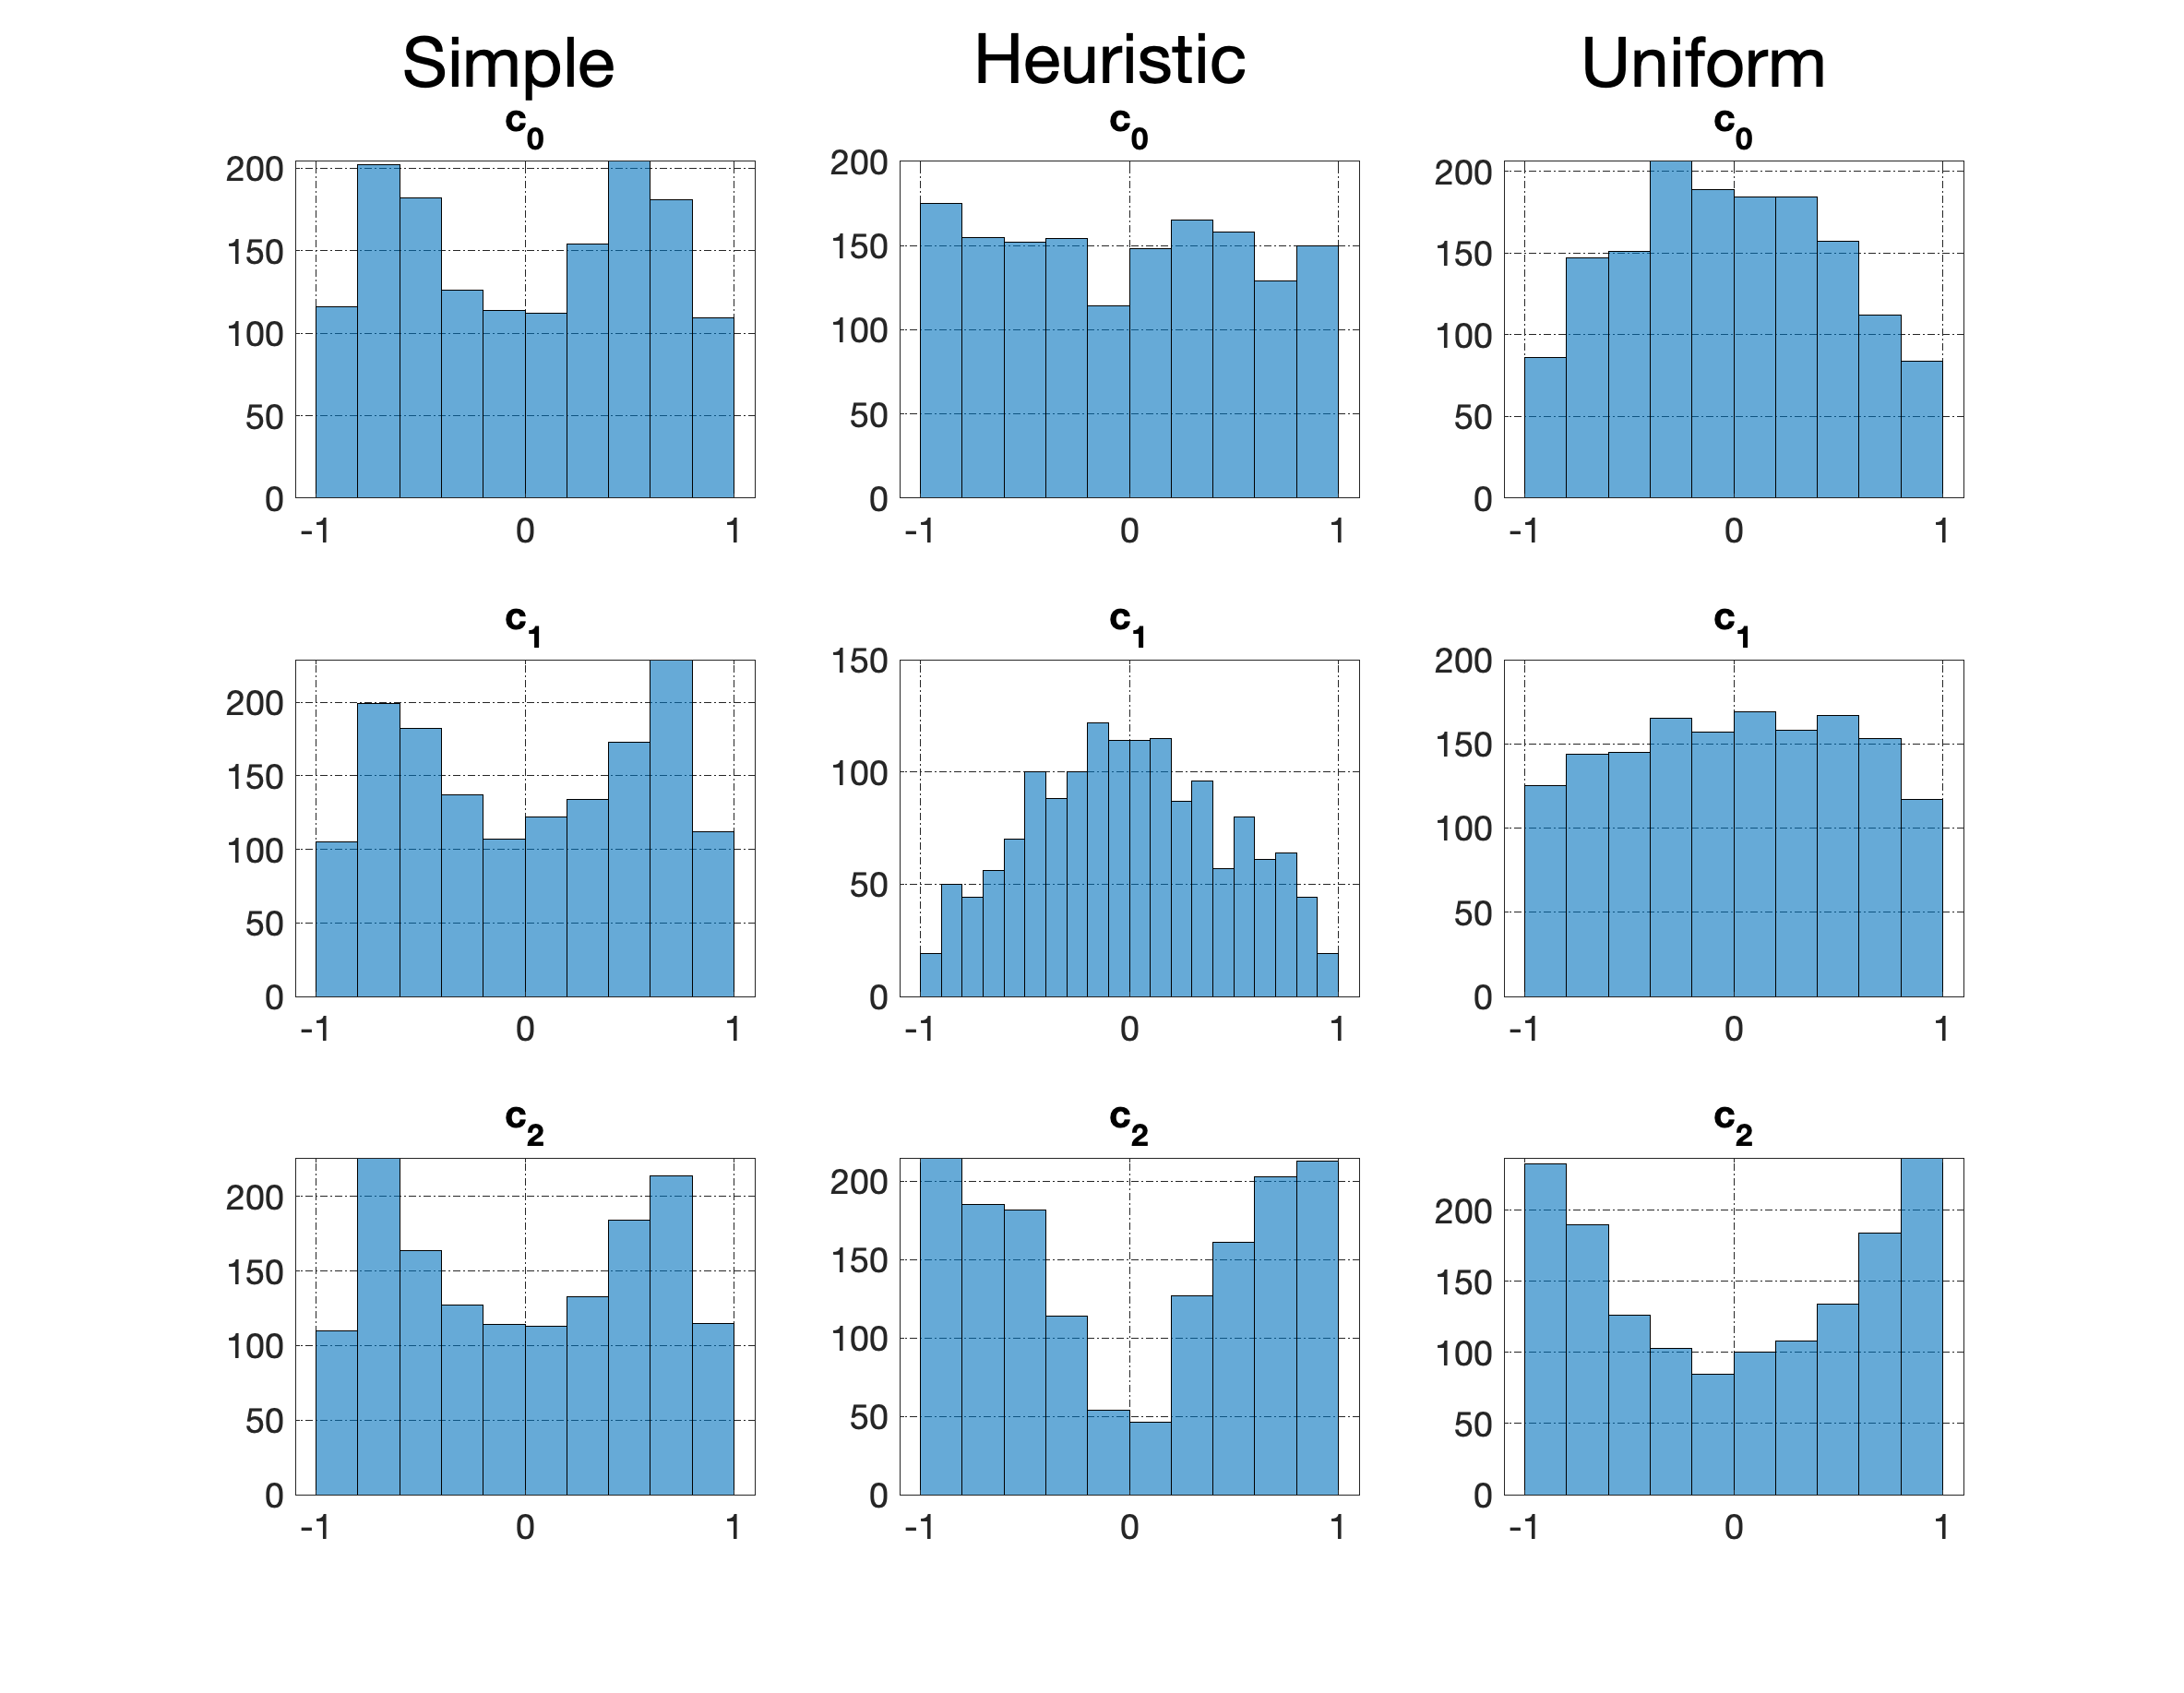
\includegraphics[width=0.5\textwidth]{images/three_coefficients_distribution.eps}
  	\caption{Распределение коэффициентов $C_i$.}
  	\label{fig:ap:three_coefficients_distribution}
  \end{figure}
  
  Пусть $l\in \mathbb{R}^{n}$ --- одна из точек, равномерно распределенных по эллипсу $\{x: x^{\top} (M M^{\top})^{-1} x \leqslant \mu \}$.
  Тогда $\widetilde{C} = M^{\top} (M M^{\top})^{-1} l + z$, где $z \in \operatorname{null}(M)$.
  
  На рисунке \ref{fig:ap:three_coefficients_distribution} приведены гистограммы распределений коэффициентов $C_i$, полученных при помощи описанных двух методов, а также восстановленных из действительно равномерно распределенных по множеству достижимости точек. 
  
  \subsection{Особенность линейных управлений}
     \begin{figure}[ht!] 
     \centering
  	\hspace{-2.5ex}
  	\begin{minipage}[b]{.4\linewidth} 
  		\small
  		\centering 
  		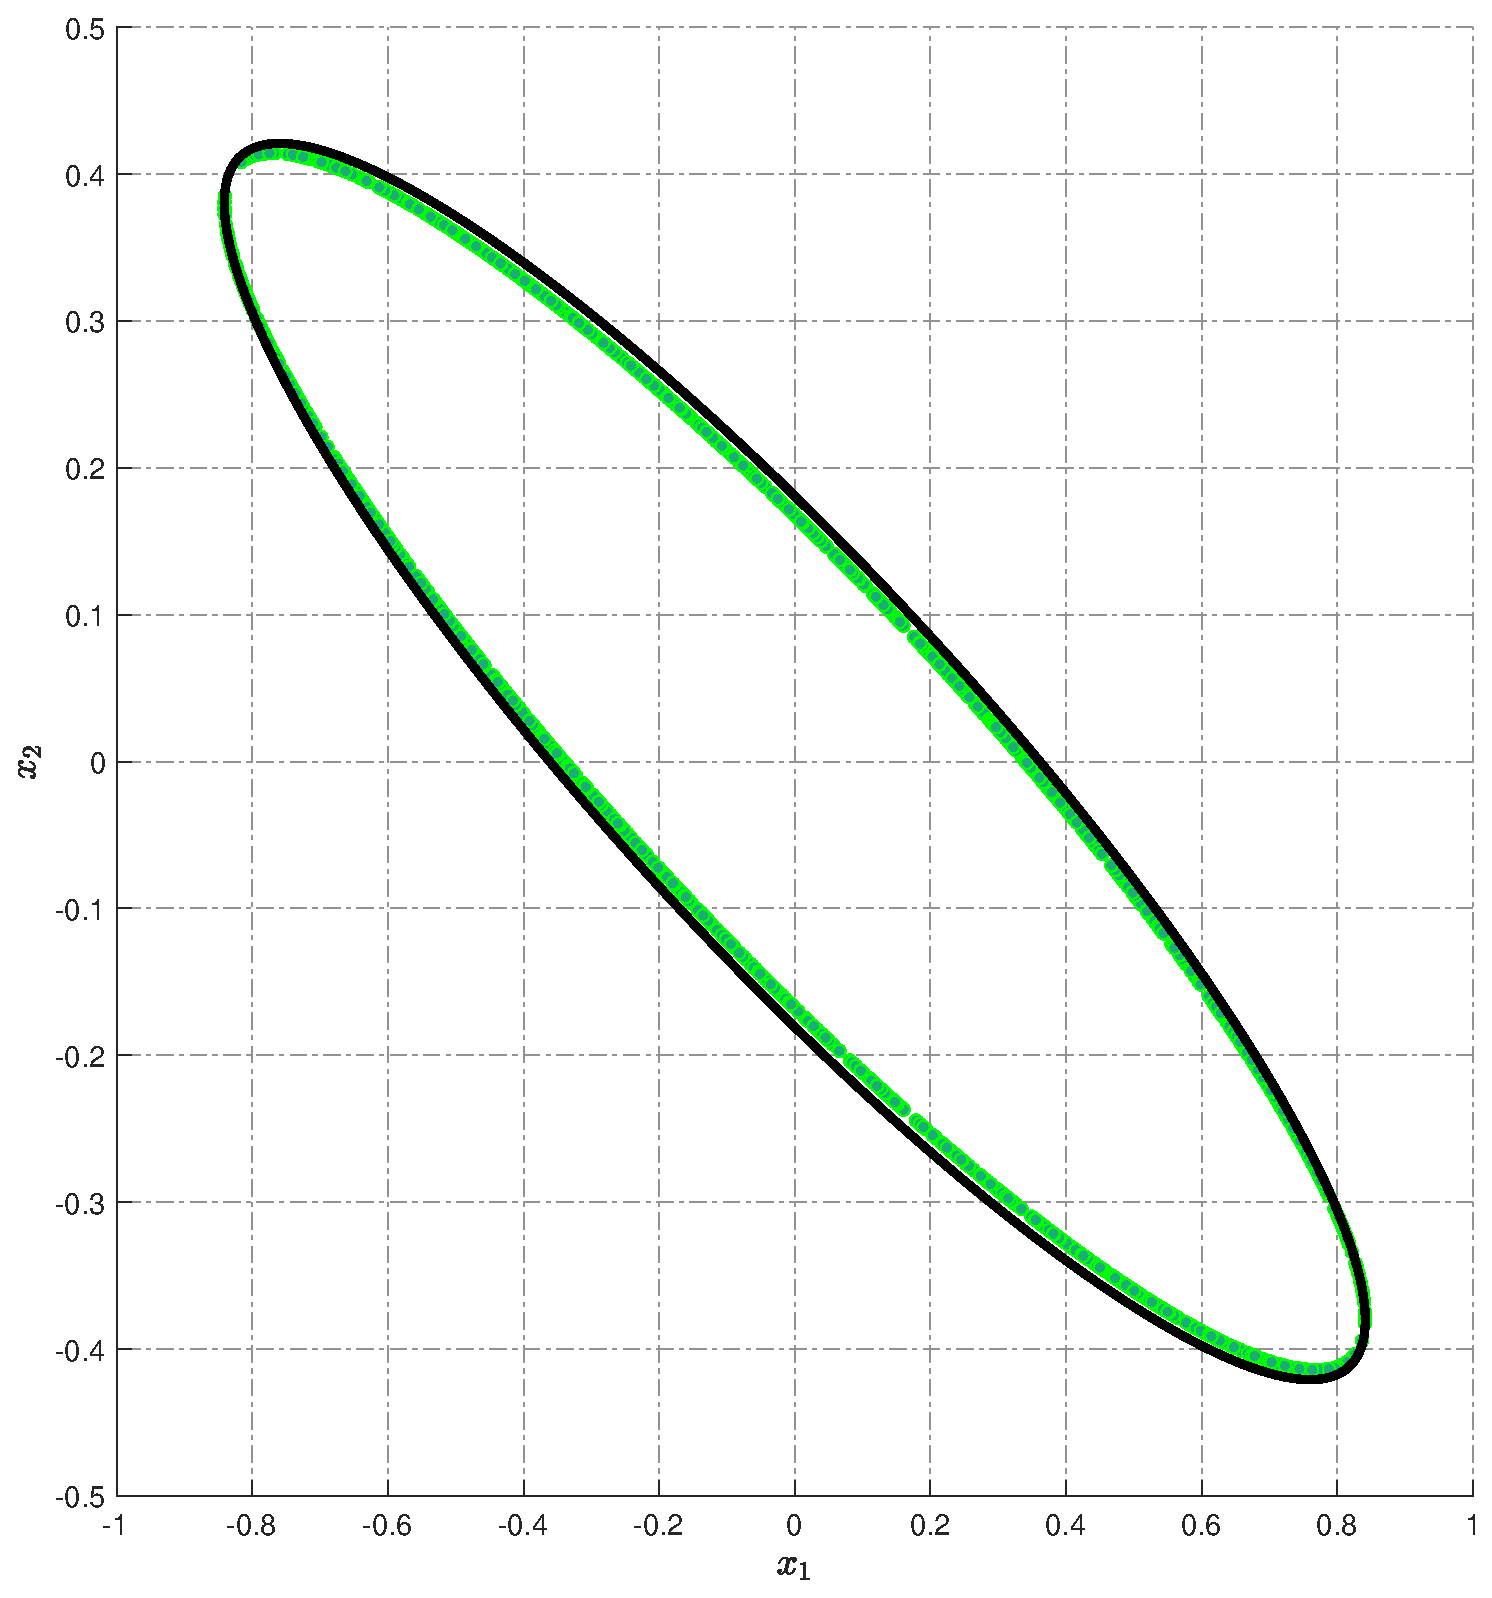
\includegraphics[width=\linewidth]{images/linear_system_linear_control.eps}
  		\subcaption{$ N = 10^3  $ } 
  		 \label{fig:ap:random_linear_system}
  	\end{minipage}
  	\hfill
  	\begin{minipage}[b]{.4\linewidth} 
  		\small
  		\centering
  		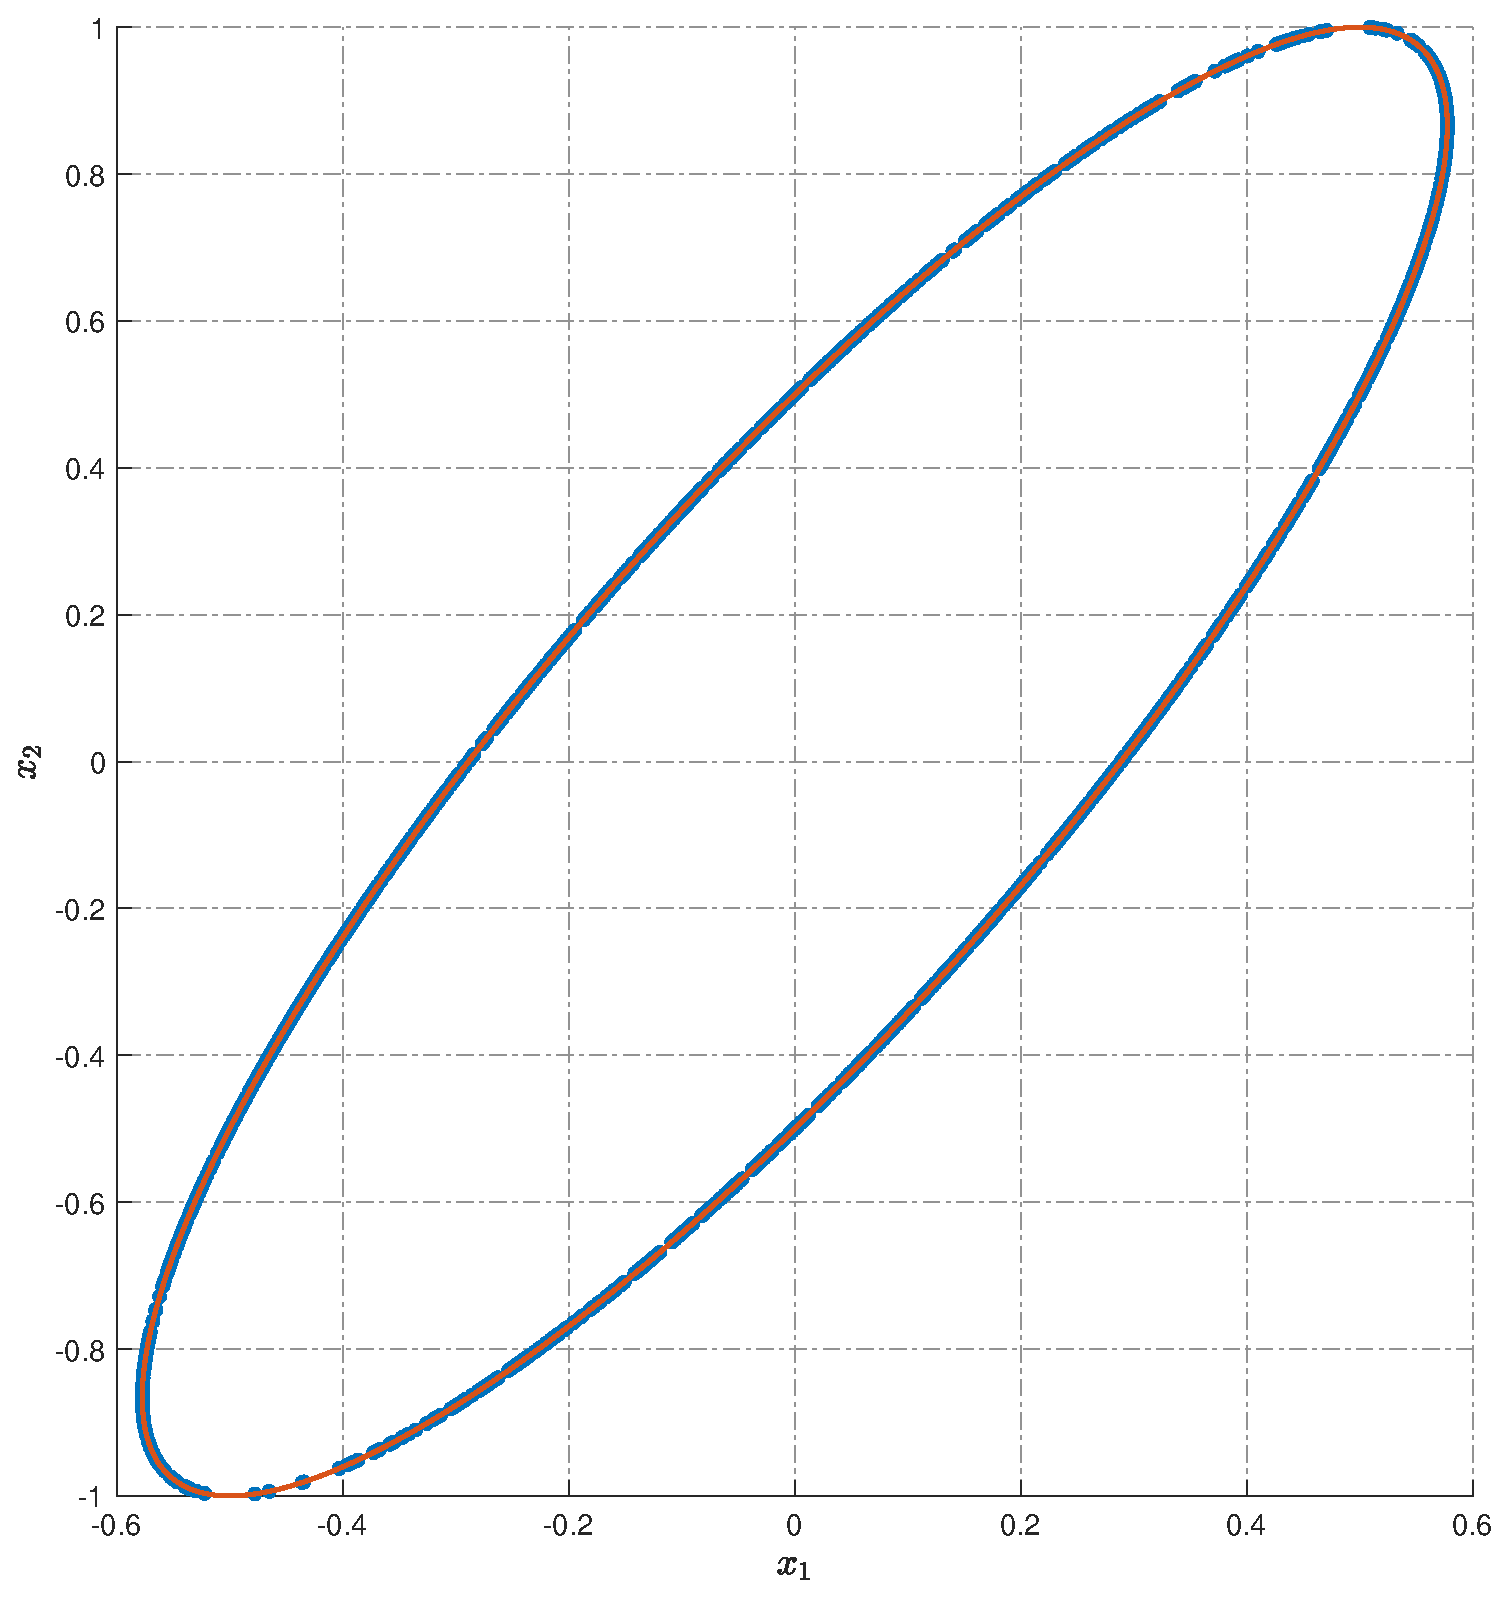
\includegraphics[width=\linewidth]{images/double_integrator_linear_control.eps}
  		\subcaption{$ N = 10^4  $ }
  		 \label{fig:ap:double_intrgrator} 
  	\end{minipage} 
  	\caption{Использование линейных управлений для линейных систем.}\label{fig:ap:linear_control}
  \end{figure}
  
  Другой особенностью, замеченной при изучении Алгоритма \ref{ap:method} является интересный эффект при использовании полиномов 1-ого порядка, то есть линейных по времени управлений, для построения множеств достижимости линейных систем.
  Точки, порождаемые такими управления, лежат на эллипсе, который очень близок к границе истинного множества достижимости (Рис.  \ref{fig:ap:random_linear_system}), а иногда и совпадает с границей (Рис. \ref{fig:ap:double_intrgrator}). 
  
  На рисунке \ref{fig:ap:random_linear_system} показано множество достижимости линейной системы
  \begin{gather}\label{ap:random_linear_system}
  	\begin{pmatrix} 
  		\dot{x}_1 \\
  		\dot{x}_2  
  	\end{pmatrix} = 
  	\begin{pmatrix}
  		0 & 1 \\
  		-2 & -3
  	\end{pmatrix}
  	\begin{pmatrix} 
  		x_1 \\
  		x_2  
  	\end{pmatrix} +
  	\begin{pmatrix} 1 \\ 0
  	\end{pmatrix} u.
  \end{gather}
  в момент времени $t = 1$, с нулевыми начальными условиями  $x_1(0) = x_2(0) = 0 $ и ограничениями на управление 
  \begin{gather*}
  	\int\limits_0^1 u^2dt \leqslant 1.
  \end{gather*}
  Используются полиномы второго порядка, то есть $u_i(t) $ линейно зависят от времени.
  
    На рисунке \ref{fig:ap:double_intrgrator} показано множество достижимости линейной системы
  \begin{gather}\label{ap:double_intrgrator}
    \dot{x}_1 = x_2,\\
  	\dot{x}_2 =  u
  \end{gather}
  в момент времени $t = 1$, с такими нулевыми начальными условиями  $x_1(0) = x_2(0) = 0 $ и такими же ограничениями на управление 
  \begin{gather*}
  	\int\limits_0^1 u^2dt \leqslant 1.
  \end{gather*}
  Как и в соседнем примере, используются полиномы второго порядка, то есть $u_i(t) $ линейно зависят от времени.
  
  Для того, чтобы понять причину этого эффекта, рассмотрим задачу оптимального управления
  \begin{gather*}
  	c^{\top} x(1) \rightarrow \max, \\
  	s.t. 	\int\limits_0^1 u^2dt \leqslant 1.
  \end{gather*}
  
  В случае системы \eqref{ap:double_intrgrator} ее решение имеет вид
  \begin{gather*}
  	u(t) = \frac{c_1(1 - t) + c_2}{\sqrt{\frac{c_1^2}{3} + c_1 c_2 + c_2^2}}, \qquad c = \big(c_1, c_2 \big)^{\top}
  \end{gather*}
  
  В случае произвольной системы $\dot{x} =Ax + Bu$ имеем
  \begin{gather*}
  	u(t) = \frac{1}{\sqrt{c^{\top}Wc}} B^{\top} \operatorname{exp}\big(-A^{\top}(1-t)\big) c,
  \end{gather*}
  где $W$ --- грамиан управляемости, $W  = \int\limits_{0}^{1}  \operatorname{exp}\big(A(1-\tau)\big) B B^{\top}  \operatorname{exp}\big(A^{\top}(1-\tau)\big) d\tau$.
  
  \subsection{Другие примеры}
  
  Для построения иллюстраций в диссертации был широко использован Алгоритм \ref{ap:method}, приведем здесь примеры некоторых систем, обладающих наиболее интересными по форме множествами достижимости.
  
   \begin{figure}[t]
   	\centering
   	\includegraphics[width=\textwidth]{images/Osipov_QuaziDuffing.eps}
   	\caption{Множества достижимости осциллятора Дуффинга \eqref{ap:Duffing}.}
   	\label{ap:fig:Duffing}
   \end{figure}
   
   \textbf{Пример 1}. На рисунке \ref{ap:fig:Duffing} показано множество достижимости системы 
   \begin{gather}\label{ap:Duffing}
   	\dot{x_1} = x_2, \qquad
   	\dot{x_2} = -x_1 - 10 \varepsilon x_1^3 + u ,
   \end{gather}
   для момента времени $t = 2$, различных значений $\varepsilon$, при нулевых начальных условиях $x_1(0) = x_2(0) = 0 $ и ограничениях на управление 
   \begin{gather}\label{ap:Duffing_controls}
   	\int\limits_0^2u^2dt \leqslant 1.
   \end{gather}
   
   \begin{figure}[ht]
   	\centering
   		\includegraphics[width=\textwidth]{images/Osipov_QuaziDubins.eps}
   	\caption{Множества достижимости системы \eqref{ap:Linear+Dubins}.}
   	\label{ap:fig:LinearDubins}
   	   \end{figure}
   	   
   	 \textbf{Пример 2}. На рисунке \ref{ap:fig:LinearDubins} показано множество достижимости системы 
   \begin{gather}\label{ap:Linear+Dubins}
   	\begin{pmatrix} 
   		\dot{x}_1 \\
   		\dot{x}_2 \\ 
   		\dot{x}_3 \end{pmatrix} = 
   	\begin{pmatrix}
   		0 & 1 & 0 \\
   		0 & 0 & 1 \\
   		0 & 0 & 0
   	\end{pmatrix}
   	\begin{pmatrix} 
   		x_1 \\
   		x_2 \\ 
   		x_3 \end{pmatrix} + 
   	\varepsilon
   	\begin{pmatrix}
   		\cos x_3 - x_2\\
   		\sin x_3 - x_3 \\
   		0
   	\end{pmatrix} + 
   	\begin{pmatrix}
   		0 \\ 0 \\ 1
   	\end{pmatrix} u.
   \end{gather}
   	для момента времени $t = 1$, различных значений $\varepsilon$, при нулевых начальных условиях$x_1(0) = x_2(0) = x_3(0) = 0 $ и таких же ограничениях на управление, как в предыдущем примере, но на интервале времени $0 \leqslant t \leqslant 1$.
   	
   	\begin{figure}[t]
   		\centering
   			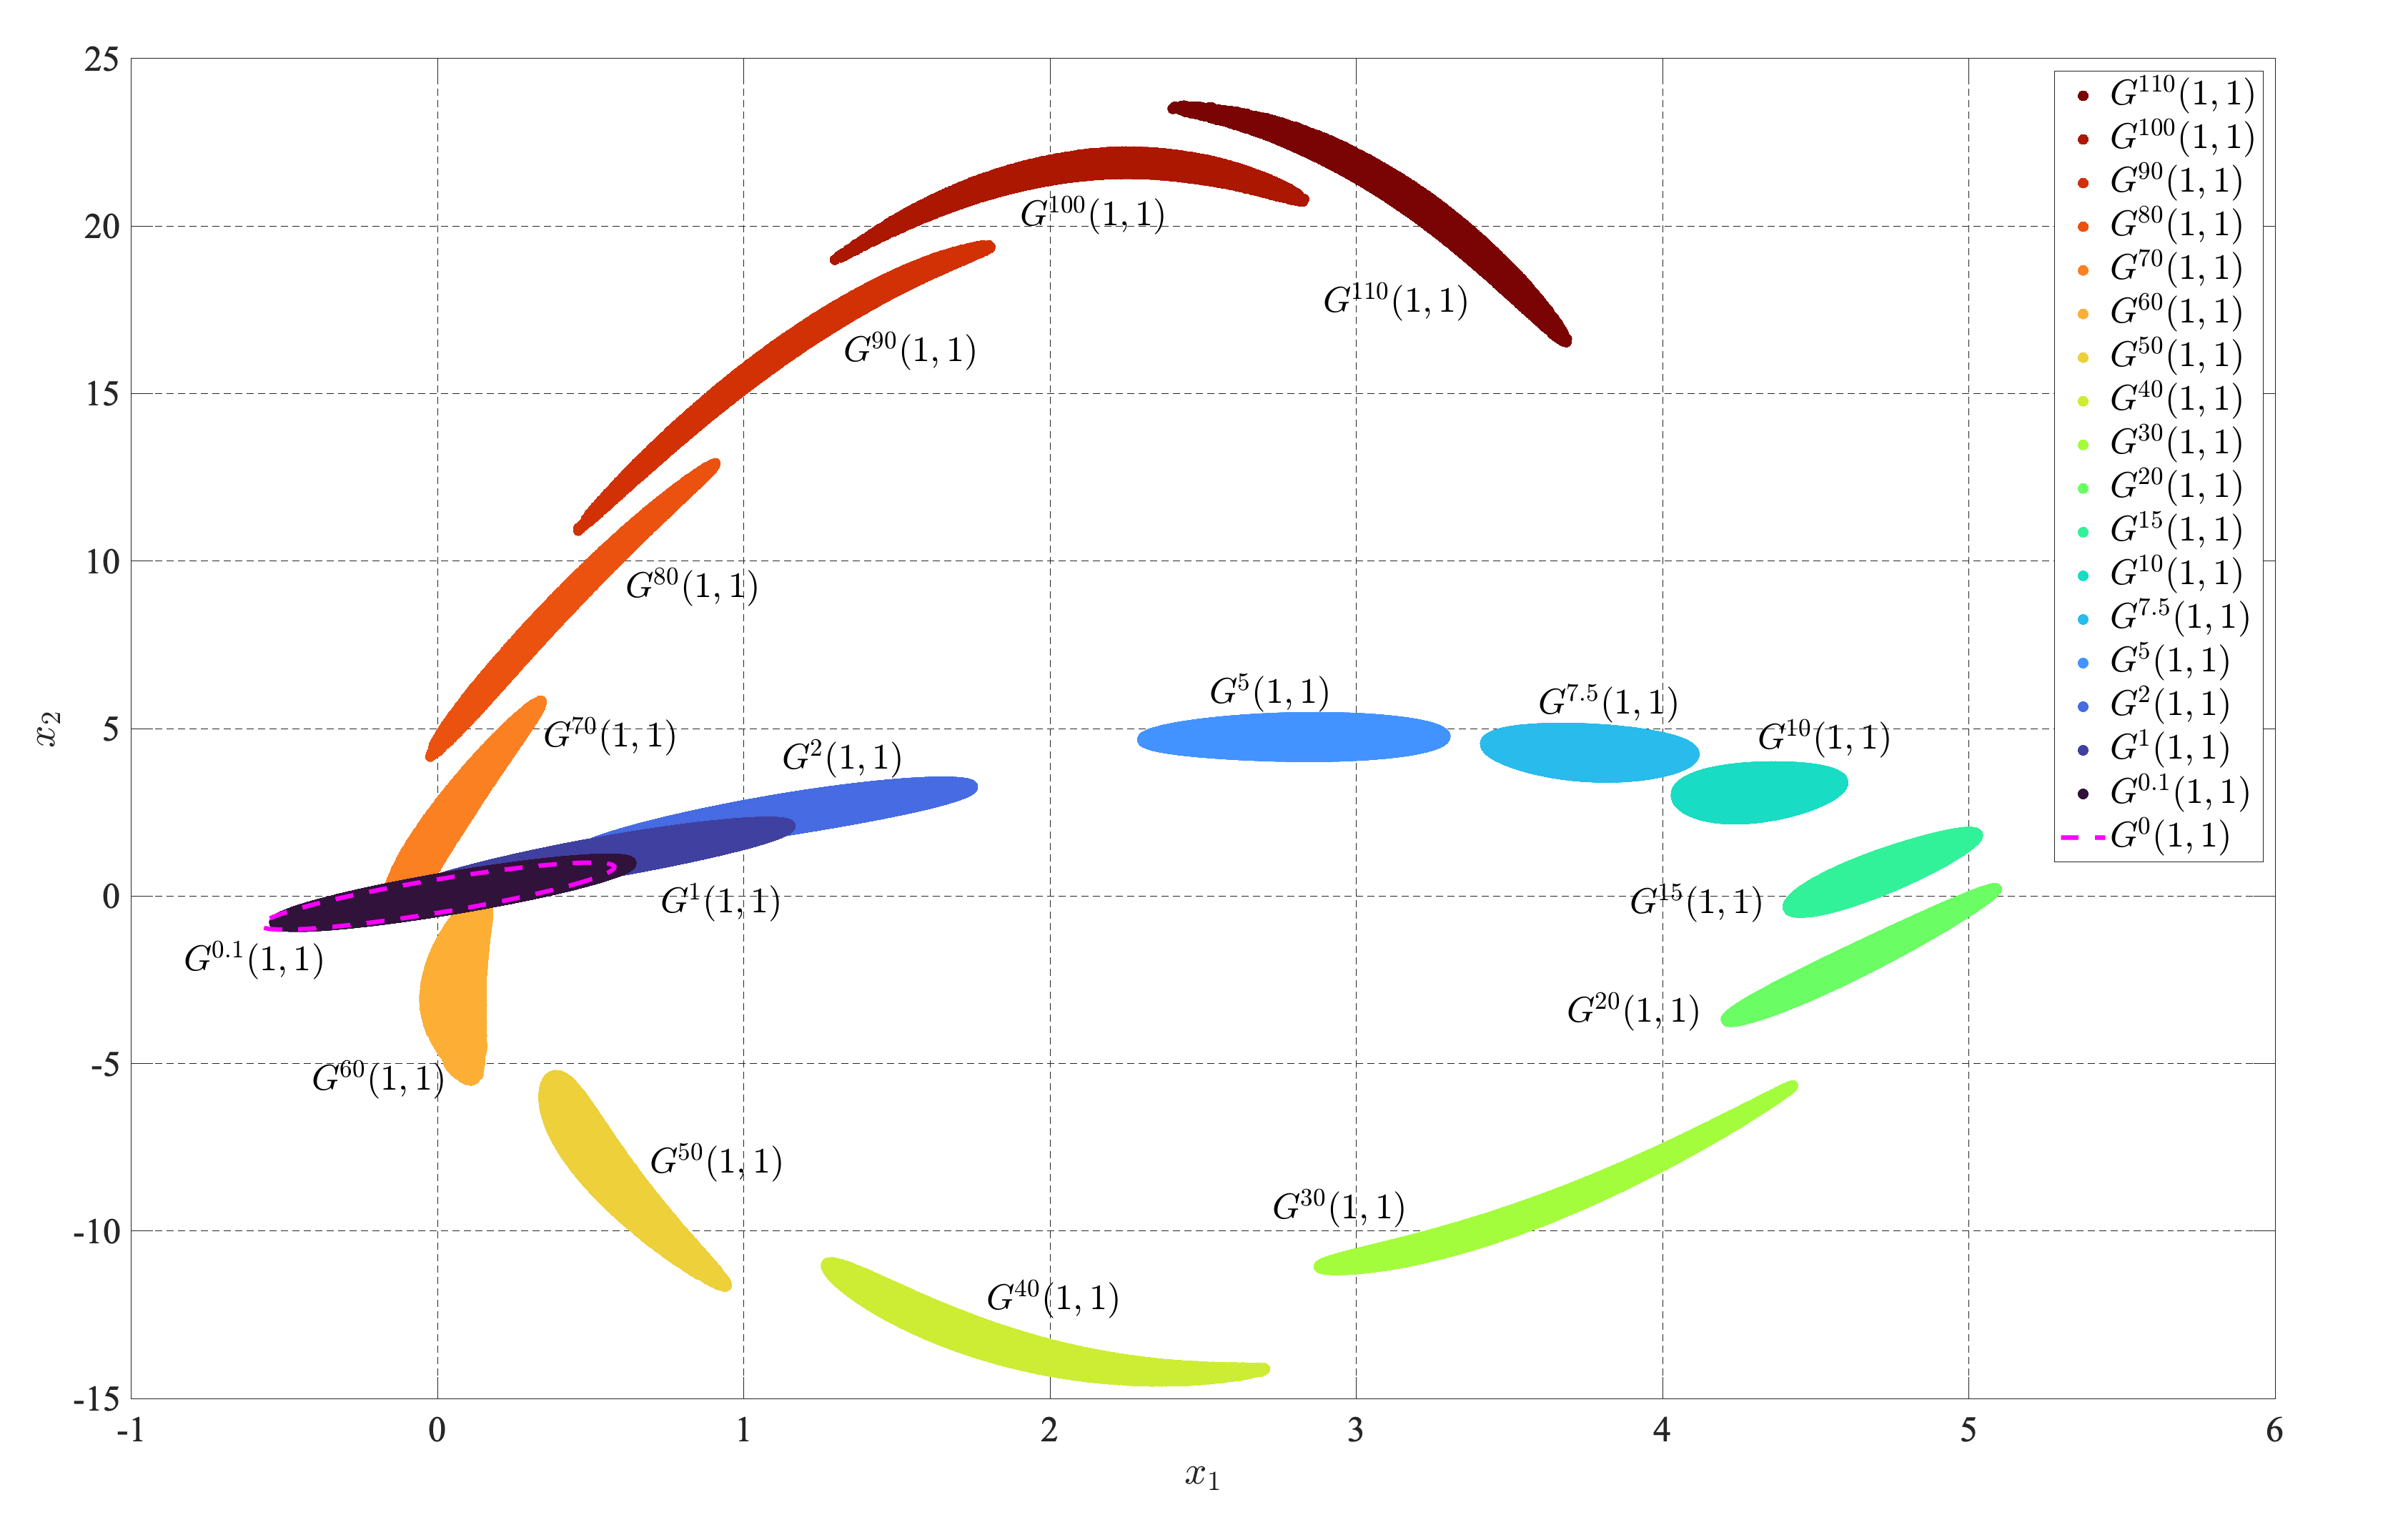
\includegraphics[width=0.92\textwidth]{images/Osipov_QuaziLinearExp.eps}
   		\caption{Множества достижимости системы \eqref{ap:Example3}.}
   		\label{ap:fig:QuaziLinearExp}
   	\end{figure}
  
   \textbf{Пример 3}. На рисунке \ref{ap:fig:QuaziLinearExp} показано множество достижимости системы 
   \begin{gather}\label{ap:Example3}
   	\dot{x_1} = x_2, \qquad
   	\dot{x_2} = u + \varepsilon(\sin x_1 + \cos x_1) ,\qquad 0\leqslant t  \leqslant 1.
   \end{gather}
   Начальное состояние $x_1(0) = x_2(0) = 0 $, управление ограничено  
   \begin{gather}\label{example3_controls}
   	\int\limits_0^1 u^2dt \leqslant 1.
   \end{gather}
  
\end{document}